\chapter{回归}
\label{chap:regression}

预测房屋价格时，可以估计平均成交价，也可以给出预算所需的上分位数或价格分布。\term{回归}（regression）根据输入估计数值响应的这些条件特征。设训练集为$D_n=\{(\bm{x}_i,y_i)\}_{i=1}^{n}$，其中$\bm{x}_i\in\mathbb{R}^{d}$为输入，$y_i\in\mathbb{R}$为响应，预测函数记为$f$；响应也可以是次数等离散数值。

需要检查变量作用或建立简洁基线时，可以从线性模型开始；关系随输入区域变化时，则考察局部回归、树或平滑函数。若决策还需要尾部阈值或分布信息，预测对象也要相应改变。

预测对象确定以后，还要选择输入与响应之间的关系。全局加权适合描述共同趋势，邻域方法在查询点附近估计响应，树与规则为不同条件分配局部预测，概率模型保留分布信息。各节沿着这些关系展开训练目标与求解过程，再考察新输入上的预测误差。第\ref{chap:classic-models-overview}章建立的建模思路，在这里由数值响应及其损失具体化。

阅读本章时可以抓住两条线索。第一条是“到底想预测响应分布的哪个位置”：默认预测条件均值，需要控制超支风险时转向条件分位数，容忍小偏差时只惩罚落在容忍带外的误差，需要完整不确定性时再估计响应分布或预测区间。预测对象不同，给误差计分的损失函数就不同。第二条是“用什么形状的函数去表示关系”：先从最容易估计也最容易解释的线性加权开始；当直线不足以描述曲率或交互时，依次尝试展开特征、参考附近样本、按条件分区，最后用概率模型描述整条函数的不确定性。本章各节正是按这两条线索的交点组织的——同一个函数表示可以搭配不同损失，同一种损失思想也能用于不同表示，因此不要把“某个模型”和“某个预测目标”混为一谈。

\section{基于线性关系的回归}
\label{sec:regression-linear}

预测房价的一个起点是给输入特征赋予权重，用加权和表示整体趋势。要由数据选出权重，就需要规定什么误差值得减小，以及多大的系数变化可以接受。最小二乘用平方残差评价拟合，正则化限制系数，分位数回归和SVR则改变误差的计分方式。原特征的线性关系不足时，还可以增加基函数或采用核；响应的取值范围与分布特征，则由GLM和GAM进一步处理。

这一小节包含的模型较多，它们其实只在回答三个依次出现的问题，按这个顺序阅读就不会迷失。第一，给定一组固定特征，怎样选出一组权重？普通最小二乘给出最基本的答案，并讨论它的两种求解方式和直线表示能力不足时的特征展开。第二，特征彼此高度相关时，最小二乘的权重会剧烈摆动怎么办？正则化通过给系数增加代价来稳定估计，成分回归则换个角度先压缩特征方向。第三，如果预测目标根本不是条件均值（要分位数、要容忍带、响应取值受限或作用本身弯曲），就要相应更换损失或响应模型，这对应分位数回归、SVR、GLM和GAM。

\subsection{普通最小二乘（OLS）}
\label{sec:regression-ols}

同一输入可能对应不同的观测响应，因而很难找到一条穿过所有样本的直线。考虑四个教学样本：$x=0$处的响应为$2,4$，$x=1$处的响应为$4,6$。两处各有两个不同数值，精确插值已经不可能；我们需要一个规则，在这些不一致的观测之间选择预测。若用平方残差计分，两个位置分别取均值$3,5$最合适，对应直线$f(x)=3+2x$。

\term{普通最小二乘}（ordinary least squares, OLS）把这种选择推广为寻找残差平方和最小的系数。平方损失让正、负误差受到相同惩罚，也让大误差付出更高代价。它可以作为无需指定响应分布的拟合准则；在独立、零均值且同方差的高斯误差下，又可解释为最大似然估计。先建立固定特征下的拟合与求解，再考察特征形状、观测精度和异常响应怎样改变这个问题\scite{bishop2006}。

\subsubsection{模型结构}
\label{sec:regression-ols-structure}

令$\bm{\phi}(\bm{x})\in\mathbb{R}^{p}$表示固定特征向量，模型写成$f_{\bm{w}}(\bm{x})=\bm{\phi}(\bm{x})^{\top}\bm{w}$，其中$\bm{w}\in\mathbb{R}^{p}$。最简单的选择是$\bm{\phi}(\bm{x})=(1,\bm{x}^{\top})^{\top}$，此时$p=d+1$，第一个系数为截距。这里的“线性”指预测对待估计系数线性；特征变换$\bm{\phi}$可以非线性，其具体形式将在本小节后面展开。

把样本堆叠为设计矩阵$\bm{X}\in\mathbb{R}^{n\times p}$，第$i$行为$\bm{\phi}(\bm{x}_i)^{\top}$，并记$\bm{y}=(y_1,\ldots,y_n)^{\top}$，得到目标
\begin{equation}
  \widehat{\bm{w}}\in\argmin_{\bm{w}}J(\bm{w}),
  \qquad
  J(\bm{w})=\frac{1}{2n}\lVert\bm{y}-\bm{X}\bm{w}\rVert_2^2.
  \label{eq:regression-ols-objective}
\end{equation}
因子$1/(2n)$不改变OLS的最优解，但会影响梯度、步长和正则系数的数值约定。本章使用平均平方损失时均沿用这一形式。

图\ref{fig:regression-ols-residuals}把这个目标放回输入与响应平面：每条虚线都是固定$x_i$之后，观测$y_i$与直线预测之间的纵向差。OLS选择的是让这些差的平方和最小的直线，因此拟合线通常不穿过每个样本；图中的距离沿响应轴测量，区别于点到直线的垂直几何距离。

\begin{figure}[htbp]
  \centering
  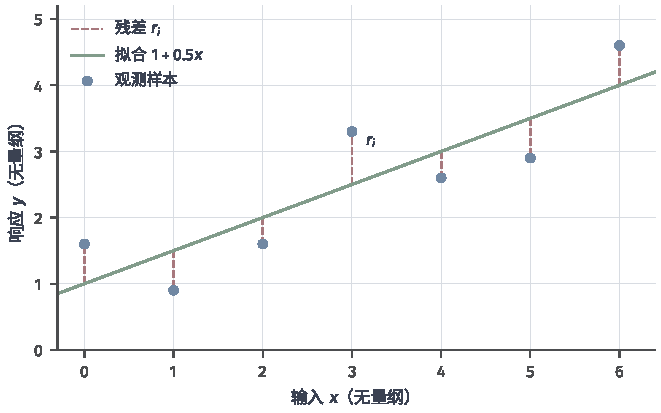
\includegraphics[width=105.412mm]{figures/04-classic-models/00-shared/matplotlib/regression-ols-residuals/figure.pdf}
  \caption{一维OLS与响应残差。七个构造样本的最小二乘直线为$\widehat f(x)=1+0.5x$；蓝色实心点表示观测，绿色实线表示预测，红色竖虚线表示$r_i=y_i-\widehat f(x_i)$。横、纵轴均为无量纲教学变量。}
  \label{fig:regression-ols-residuals}
\end{figure}

手中的残差平方和只评价已经观测到的记录。需要提醒的是，把训练误差压到零并不难，也往往不是目的：只要模型足够灵活（比如让一条折线穿过每个训练点），训练误差就能为零，但这条折线在任意两个训练点之间的取值毫无依据，换一批数据得到的折线也完全不同。若要判断预测函数面对未来记录时怎样，就要按未来输入与响应的共同分布，计算平方损失的平均值$\mathbb E[(Y-f(\bm X))^2/2]$；这种未来平均损失称为期望风险（expected risk）。先固定一个输入$\bm x$，把该输入处的条件均值记为$m(\bm x)=\mathbb E[Y\mid\bm X=\bm x]$。对任意实数预测$a$，条件平方误差可拆成
\[
 \begin{aligned}
 &\mathbb E[(Y-a)^2\mid\bm X=\bm x]\\
 &\quad=\operatorname{Var}(Y\mid\bm X=\bm x)
             +[m(\bm x)-a]^2.
 \end{aligned}
\]
第一项是固定输入后响应自身的波动，不随$a$改变；第二项在$a=m(\bm x)$时最小。再按未来输入出现的频率平均，就解释了平方损失为何以条件均值为预测目标，而不是以每条带噪响应为必须穿过的点。

响应二阶矩有限时，条件均值在平方可积预测函数中达到最小风险，且只在输入分布的几乎处处意义下唯一，可参考\BookChapterRef{chap:random-variables}{卷二《数学准备：概率、因果与决策》的“随机变量”章}。
限制为$f_{\bm w}$以后，若条件均值不属于所选模型类，OLS估计的只是该类中的平方逼近；
高斯性、同方差性与误差对称性都不是平方损失以条件均值为目标的必要条件。
这里的平方可积要求函数值的平方具有有限期望。“几乎处处”允许函数在输入概率为零的集合上不同，因为这种差异不会改变上述平均损失。总体中的最佳候选与有限数据算出的系数仍有区别：OLS用训练记录的平均损失估计这个总体目标，某一次样本得到的最优函数未必就是总体中最近的候选。

\subsubsection{参数学习}
\label{sec:regression-ols-learning}

OLS的参数学习有两条路线。一条路线直接求出最优系数的方程，再用矩阵分解解方程；另一条路线从初始系数出发，反复减小训练损失。

先看第一条：式\eqref{eq:regression-ols-objective}是一个无约束、可微的凸二次目标。“凸”意味着它的等高线像碗的内壁，从任意点沿碗壁向下走都不会掉进某个只在局部最低的小坑；因此只要找到坡度恰好为零的位置，就能确认这是全局最低点，而不必担心别处还有更低的解。在最小点处，每个系数方向上的一阶变化都应为零。对残差平方求导得到
\[
  \nabla J(\bm w)=\frac1n\bm X^\top(\bm X\bm w-\bm y),
  \qquad \nabla^2J(\bm w)=\frac1n\bm X^\top\bm X.
\]
第二个矩阵半正定，说明目标凸；因此梯度为零不仅是必要条件，也足以认证全局最优。把第一式置零，就得到\term{正规方程}（normal equations）。它要求残差与每一列特征正交：沿任何已提供的特征方向调整系数，都不能再降低平方误差。
\begin{equation}
  \bm{X}^{\top}\bm{X}\widehat{\bm{w}}=\bm{X}^{\top}\bm{y}.
  \label{eq:regression-normal-equations}
\end{equation}

若$\bm X\bm v=\bm0$，将$\bm v$加到系数上不会改变训练预测。所有这类向量组成设计矩阵的零空间，记为$\operatorname{null}(\bm X)$。还可以在全部最小二乘解中选择长度最小的代表，写为$\bm X^\dagger\bm y$；符号$\dagger$表示Moore--Penrose伪逆（Moore--Penrose pseudoinverse），它在这里把响应向量送到这个最小范数代表。解集因而可以读成“一个代表加上任意训练不可见的方向”。

正规方程的全部参数解为$\bm X^\dagger\bm y+\operatorname{null}(\bm X)$，可参考\BookChapterRef{chap:linear-algebra-and-matrix-analysis}{卷一《数学准备：计算、分析与几何》的“线性空间”章}。
因此训练拟合值总是唯一，参数唯一则要求设计矩阵列满秩；否则可取最小范数解。
零空间中的参数差在训练点上不可见，却可能在新特征向量上产生不同预测。

闭式表达用于分析，计算时通常不显式求逆。列满秩且$n\geq p$时，薄QR分解$\bm{X}=\bm{Q}\bm{R}$把问题化为三角方程$\bm{R}\widehat{\bm{w}}=\bm{Q}^{\top}\bm{y}$，稠密计算代价约为$O(np^2)$。

这里$\bm Q\in\mathbb R^{n\times p}$的列是标准正交的，满足$\bm Q^\top\bm Q=\bm I_p$；$\bm R\in\mathbb R^{p\times p}$为可逆上三角矩阵。“薄”表示只保留张成训练列空间所需的$p$列。把响应分成该空间内外两部分，就有
\[
 \begin{aligned}
 \lVert\bm y-\bm Q\bm R\bm w\rVert_2^2
 &=\lVert\bm Q^\top\bm y-\bm R\bm w\rVert_2^2\\
 &\quad+\lVert(\bm I_n-\bm Q\bm Q^\top)\bm y\rVert_2^2.
 \end{aligned}
\]
第二项不随系数改变，第一项可以令其为零，所以只需回代求解上述三角方程。这条路线没有先把设计矩阵乘成正规方程矩阵。

奇异值分解（singular value decomposition，SVD）则把设计写成$\bm X=\bm U_r\bm D_r\bm V_r^\top$，其中$r$为秩，$\bm U_r$与$\bm V_r$各有$r$列标准正交向量，$\bm D_r$的对角元$s_1,\ldots,s_r$为正奇异值。系数空间中的方向$\bm v_j$经过设计矩阵后满足$\bm X\bm v_j=s_j\bm u_j$：$\bm u_j$位于训练预测空间，$s_j$表示系数沿该方向改变时，训练预测被放大多少。奇异值很小，就意味着较大的系数变化只产生较小的训练变化；零空间方向则完全不可见。
最小范数解因此可以按各方向直接计算：
\[
 \bm X^\dagger\bm y
 =\sum_{j=1}^r\frac{\bm u_j^\top\bm y}{s_j}\bm v_j.
\]
先把响应投到$\bm u_j$方向，再除以该方向的放大倍数$s_j$，就还原对应系数；训练不可见的零空间分量取零。小$s_j$也会放大响应中的噪声，这正是病态方向难以估计的原因。

秩亏或需要检查小奇异值时可以用SVD。直接形成$\bm{X}^{\top}\bm{X}$会把满列秩矩阵的二范数条件数平方，因此近似共线时尤其应避免求逆实现。
满列秩时，这个条件数是最大与最小奇异值之比$s_{\max}/s_{\min}$，衡量不同方向的尺度差别。$\bm X^\top\bm X$的特征值变为$s_j^2$，其极端值之比于是变成原比值的平方；很弱的方向因而会使正规方程对数据与舍入误差更敏感。

第二条路线适合不便一次完成矩阵分解的规模。我们从$\bm w^{(0)}$出发，沿训练损失的负梯度调整系数：
\begin{equation}
  \bm{w}^{(t+1)}
  =\bm{w}^{(t)}+\frac{\eta}{n}
       \bm{X}^{\top}(\bm{y}-\bm{X}\bm{w}^{(t)}).
  \label{eq:regression-ols-gradient}
\end{equation}
非零设计下令$L=\lambda_{\max}(\bm X^\top\bm X/n)>0$，可以取$\eta=1/L$。沿第$j$个正特征值方向，系数误差每轮乘$1-\eta s_j^2/n$，这个选择使各因子位于$[0,1)$；小奇异值方向仍会收缩得慢。秩亏时零空间分量保持初值，从零启动则选出最小范数解。若设计全零，目标不随系数改变，无需迭代；一般停止时检查目标变化和梯度残差。

一次完整更新需要$O(np)$次算术操作；使用大小为$b$的小批量时，一次梯度估计需$O(bp)$，但总更新次数和随机误差也须考虑。代码\ref{code:regression-ols}展示矩阵求解接口与预测；截距列需由调用者加入，返回的秩可用于检查参数是否可识别。

\begin{codeblock}[language=Python,label={code:regression-ols},unbreakable]{用最小二乘接口求解并预测}
import numpy as np

# X: (n, p), y: (n,), X_new: (n_new, p)
# 截距列与特征变换在训练、预测时保持一致。
w, residuals, rank, singular_values = np.linalg.lstsq(
    X, y, rcond=None
)
y_pred = X_new @ w
\end{codeblock}

\subsubsection{特征展开：从直线到局部曲线}
\label{sec:regression-ols-theory}
\label{sec:regression-basis}

求出系数并不能补上输入表示中缺少的变化。若特征只有$1,x$，候选只能是直线；加入$x^2$后，才允许二次曲线。例如$X$在$[-1,1]$上均匀分布、条件均值为$m(x)=x^2$时，最佳直线是常数$1/3$，仍无法同时贴合中部与两端。对称性使最佳斜率为零，而$\mathbb E[X^2]=1/3$、$\mathbb E[X^4]=1/5$给出半平方误差
\[
 \frac12\mathbb E[(X^2-1/3)^2]
 =\frac12\left(\frac15-\frac19\right)=\frac{2}{45}.
\]
加入二次特征以后，系数$(0,0,1)$就能表示这个目标。图\ref{fig:regression-feature-approximation}比较的是两个候选空间的最佳函数，不是两次训练误差。

\begin{figure*}[htbp]
  \centering
  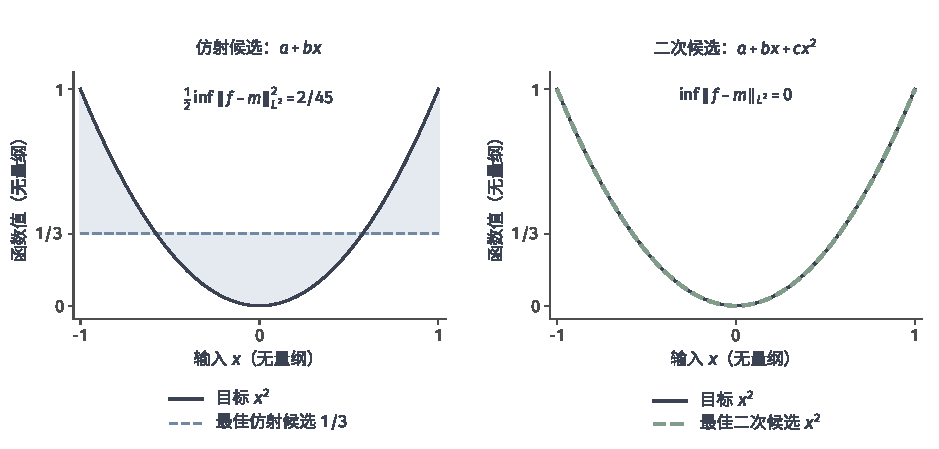
\includegraphics[width=159mm]{figures/04-classic-models/00-shared/matplotlib/regression-feature-approximation/figure.pdf}
  \caption{固定目标$m(x)=x^2$与不同候选空间的最佳逼近。输入在$[-1,1]$上均匀分布；左图中，所有仿射函数的最佳候选为$1/3$，阴影表示它与目标的差距，平方距离的一半为$2/45$。右图加入二次特征后，候选空间包含目标，最小距离为零。图中比较的是候选空间，不使用训练样本。}
  \label{fig:regression-feature-approximation}
\end{figure*}

选择新的特征向量$\bm\phi(\bm x)$以后，模型仍对系数线性，学习仍使用同一个最小二乘目标，改变的是设计矩阵的列。多项式使用$1,x,\ldots,x^q$；径向基$\exp(-(x-c_j)^2/(2s^2))$在中心$c_j$附近产生局部起伏，$s>0$决定作用范围。固定中心与尺度后，只需学习各基函数的加权系数；若也要选择这些位置与尺度，应在训练折内完成并用验证误差比较。

样条用分段多项式描述局部变化，并约束相邻段如何连接。结点$\xi_1,\ldots,\xi_K$是分段接合的位置。三次样条要求函数值和前两阶导数在结点两侧连续，可以用$1,x,x^2,x^3$及$(x-\xi_k)_+^3$展开，其中$(a)_+=\max(a,0)$。全局三次项给出左侧起始曲线，截断项从各自结点起改变右侧形状；它在结点处的函数值和前两阶导数都为零，因而保留接合条件。只用截断项会遗漏一般的全局多项式部分。

增加基函数能提供新的曲线形状，也会增加待估系数并可能加重共线性。下面先看观测误差结构与异常响应怎样改变拟合，再用正则化控制系数。核方法则把显式特征的内积换为核值计算，相关回归形式见第\ref{sec:regression-kernel-svr}节\scite{hastie2009}。

\subsubsection{观测精度与异常响应}

\paragraph{利用观测误差结构}
\label{sec:regression-weighted-noise}

观测精度不同，平方残差也未必应受到相同权重。假设两次独立观测测量同一个未知常数，噪声方差分别为$1$和$100$。OLS直接取两次观测的平均；用噪声方差倒数加权，则给第一条观测$100$倍于第二条的权重，降低较不精确观测的影响。

更一般地，已知正定误差协方差$\bm\Omega$时，最小化$(\bm y-\bm X\bm w)^\top\bm\Omega^{-1}(\bm y-\bm X\bm w)$得到\term{广义最小二乘}（generalized least squares, GLS）。它按噪声结构重新度量残差，对角$\bm\Omega$对应加权最小二乘，用$\bm\Omega^{-1/2}$变换数据即可回到同方差问题。异方差在零条件均值下不破坏OLS无偏性，却会改变其协方差，因此这种调整服务于估计方差；若$\bm\Omega$也要由样本估计，还要计入协方差估计的误差。

这个变换必须同时施于响应与全部特征。取对称正定逆平方根$\bm C=\bm\Omega^{-1/2}$，令$\bm y'=\bm C\bm y$、$\bm X'=\bm C\bm X$，就把观测方程变成$\bm y'=\bm X'\bm w+\bm C\bm\varepsilon$。新误差的协方差为$\bm C\bm\Omega\bm C^\top=\bm I_n$，因此这种消除噪声尺度与相关性的操作称为白化（whitening）。变换后的普通残差平方和$\lVert\bm y'-\bm X'\bm w\rVert_2^2$恰好等于原来的协方差加权目标。对角$\bm\Omega$只要求把第$i$条记录的响应与每个特征一起除以其误差标准差；非对角时还会混合不同记录，从而消除误差相关。随后对$(\bm X',\bm y')$使用前述QR或SVD求系数，再在原特征上计算$\bm\phi(\bm x)^\top\bm w$；白化改变了训练准则，并未改变新输入的预测公式。

\paragraph{限制异常响应的影响}
\label{sec:regression-huber}

如果少数响应记录受到污染，而预测仍面向未受污染的数据，追随这些记录就可能把拟合偏离真正的预测目标。限制污染记录的影响是改善泛化的一条思路；若极端响应本来就是目标分布的一部分，则还需检查这种限制是否符合所用损失和预测目标。

平方损失把十倍残差变成一百倍损失，少量错误记录因此可能主导拟合。只拟合一个常数时，构造响应$(0,0,0,20)$的OLS预测为$5$；最后一个大响应把预测从前三个样本所在的零点拉开。若希望保留小误差处的平滑拟合，又减轻大残差的作用，可以让损失在离零较远处按残差绝对值增长。

\term{Huber损失}（Huber loss）采用这一做法：小残差处保持二次形状，大残差处改为线性增长，从而限制残差方向的导数。取下式阈值$\delta=1$，刚才四个响应的最优常数变成$1/3$；三个小残差共同抵消最后一个被截断的残差导数。它来自稳健位置估计的研究，也可用于回归目标\scite{huber1964}。
\begin{equation}
  \rho_\delta(r)=
  \begin{cases}
    r^2/2,&|r|\leq\delta,\\
    \delta|r|-\delta^2/2,&|r|>\delta,
  \end{cases}
  \qquad\delta>0.
  \label{eq:regression-huber-loss}
\end{equation}
对$r_i=y_i-\bm{\phi}(\bm{x}_i)^{\top}\bm{w}$最小化$\sum_i\rho_\delta(r_i)$，估计方程为$\sum_i\bm{\phi}(\bm{x}_i)\psi_\delta(r_i)=\bm{0}$，其中$\psi_\delta(r)=\max(-\delta,\min(r,\delta))$。令$a_i=\min(1,\delta/|r_i|)$，在$r_i=0$时取$a_i=1$，便可交替计算残差权重与加权最小二乘；应检查目标和估计方程的收敛。阈值$\delta$具有响应单位，常结合稳健尺度估计选择；采用中位绝对偏差定标时，还需按误差分布校准所用倍数。

这个权重使$\psi_\delta(r_i)=a_i r_i$。具体求解时，从当前系数算出残差，再由这些残差算出$a_i$；本轮暂时固定权重，最小化$\sum_i a_i(y_i-\bm\phi(\bm x_i)^\top\bm w)^2$，其正规方程就使用加权残差$a_i r_i$。新系数会改变残差和权重，因此必须重新计算并重复，这就是反复加权最小二乘（iteratively reweighted least squares，IRLS）的闭环，不能只用一次OLS残差定权后便当作Huber解。停止时还要核对原Huber目标和原估计方程，而不只比较两轮系数的变化。

前面的常数算例也可在这个方程中复算。设常数预测为$a$，$\delta=1$；在$0\leq a\leq1$内，三个零响应的残差导数都是$-a$，响应$20$的残差导数则为$1$，所以估计方程为$-3a+1=0$，给出$a=1/3$。它确实落在所用分段内，凸性保证该驻点为全局最小点。用于选择阈值的中位绝对偏差（median absolute deviation，MAD）则是$\operatorname{median}_i|r_i-\operatorname{median}_j r_j|$；它给出稳健的残差尺度，不能替代阈值在目标误差分布下的校准。

将一般残差函数$\rho$代入$\min_{\bm{w}}\sum_i\rho(r_i)$，便得到以回归参数为目标的\(M\)估计（M-estimation）。Huber准则凸且连续可微；Tukey双权、Cauchy等准则则可能非凸，求解与统计性质须分别分析。估计方程中的样本贡献是特征向量与$\psi_\delta$的乘积。有界残差导数限制了响应方向的影响，但远离其他输入的高杠杆点仍可因特征幅度较大而主导估计。Huber准则拟合的是自身损失下的最优中心；条件分布偏斜时，令截断残差导数平均为零所得到的中心可能偏离条件均值。因此应按Huber损失及任务需要验证预测，不能将残差降权直接当成条件均值平方风险的改善保证。

\subsection{正则化线性回归}
\label{sec:regression-regularization}

面积与套内面积高度相关时，许多系数组合能产生近似相同的训练预测，数据却难以分辨它们。把情形简化为两列特征完全相同，预测就只取决于$w_1+w_2$；$(100,-98)$与$(1,1)$在训练点上给出同样结果。到了两列略有差别的新输入$(1.01,1)$，两组系数的预测却分别为$3$与$2.01$。较大的相反系数把训练中几乎看不到的差异放大了。

\term{正则化}（regularization）在拟合准则中加入参数约束或惩罚，让这种缺少数据支持的变化也付出代价。直观地说，在训练集上几乎无法区分的两组系数，我们倾向于选数值更小、更“不极端”的那一组，因为大的相反系数相当于在数据很少看到的方向上押了重注，新样本稍有不同就会被放大成预测剧变。它可以减少估计的波动，但系数被压小也可能连带压低真实信号。因此，正则化的用途是用可接受的偏差换取较小的方差，是否改善未来预测仍取决于真实结构、正则强度和测试分布。

\subsubsection{模型结构}
\label{sec:regression-penalties}

本小节将截距$b$与斜率$\bm{w}\in\mathbb{R}^d$分开。平方损失下，固定斜率的最优截距为$b=\bar y-\bar{\bm{x}}^{\top}\bm{w}$，所以可先用训练均值中心化特征与响应，只优化斜率，再恢复截距。以下$\bm{X},\bm{y}$均指中心化后的量，截距不受惩罚；需要标准化时，尺度也只能从训练集估计。

四种常见方法都在$\lVert\bm{y}-\bm{X}\bm{w}\rVert_2^2/(2n)$之外增加凸惩罚。\term{岭回归}（ridge regression）使用$\lambda\lVert\bm{w}\rVert_2^2/2$抑制参数幅度，收缩数据约束较弱的方向。Hoerl与Kennard在1970年的论文中系统研究了非正交设计下的有偏估计：当共线性使OLS方差过大时，容许一定偏差可能换来较小的均方误差\scite{hoerl1970ridge}。

岭回归通常保留每个变量，只把系数变小。如果记录了许多特征，而我们还希望删去缺乏预测作用的坐标，就需要让某些系数恰好为零。\term{Lasso}（least absolute shrinkage and selection operator）使用$\lambda\lVert\bm w\rVert_1$实现这种选择。绝对值惩罚在零点有尖点，损失项对某个坐标的推动较弱时，最优系数可以停在零点。比如正交标准化设计下，OLS系数为$(0.12,1.40)$，取$\lambda=0.20$后Lasso得到$(0,1.20)$；岭回归在同一数值的惩罚系数下则得到$(0.10,1.40/1.20)$，两个坐标都保留。这里比较的是两种惩罚的作用方式，不代表相同数值的$\lambda$给出相同强度的约束。Tibshirani在1996年提出Lasso，将连续收缩与变量选择放进同一个优化问题\scite{tibshirani1996lasso}。

这个教学设计的“正交标准化”具体指中心化后$\bm X^\top\bm X/n=\bm I_d$：不同列的样本内积为零，每列平方长度为$n$。于是每个坐标都有相同的数据曲率，坐标之间没有交叉项；Lasso分别将OLS系数向零移动$\lambda$并截断，岭回归则分别除以$1+\lambda$。上面的数值由这两种操作直接得到；后面将从最优性条件说明软阈值的来由。

Lasso的坐标选择在特征高度相关时也会出现歧义。若两列完全相同，并且最优系数和为正，$(a,0)$、$(0,a)$与$(a/2,a/2)$具有同样的数据拟合和一范数惩罚。数据难以决定该保留哪个变量，轻微扰动就可能改变选择。\term{弹性网}（elastic net）在一范数之外加入二次惩罚；上面三种分配中，平均分摊的平方范数最小。它因此同时保留坐标选择和稳定相关系数的机制。惩罚写成$\lambda_1\lVert\bm w\rVert_1+\lambda_2\lVert\bm w\rVert_2^2/2$，常取$\lambda_1=\lambda\alpha$、$\lambda_2=\lambda(1-\alpha)$，其中$0\leq\alpha\leq1$。Zou与Hastie在2005年研究了这一结合；原始文献还讨论了对系数重标定以修正过度收缩的版本\scite{zou2005elastic}。

另一些变量由多个系数共同表示。例如用$t,t^2,t^3$表示楼龄作用，三个坐标合起来才是一个楼龄函数；我们的选择问题可能是“是否保留楼龄”，而不是“是否保留某次幂”。\term{组Lasso}（group Lasso）把预先指定的一组坐标作为一个选择单位，使用惩罚$\lambda\sum_{g=1}^{G}\omega_g\lVert\bm w_{A_g}\rVert_2$。其中$A_1,\ldots,A_G$是不重叠且覆盖全部斜率坐标的组，$\omega_g>0$为组权重，常取$\sqrt{|A_g|}$。组向量为零，就意味着这一整组的作用被删除；保留一组则允许各系数共同拟合其形状，组内的某些坐标仍可为零。Yuan与Lin在2006年研究了这种成组变量选择，包括分类特征展开的多个指示变量\scite{yuan2006group}。

表\ref{tab:regression-regularization-comparison}将四种方法放在相同的平方损失下比较。选择方法时，需要区分“系数整体变小”“某个坐标变零”和“某组变量一起变零”；这三种要求对应不同的结构假设。

\begin{table*}[t]
  \centering
  \small
  \setlength{\tabcolsep}{4pt}
  \renewcommand{\arraystretch}{1.25}
  \begin{tabularx}{\linewidth}{@{}>{\RaggedRight\arraybackslash}p{16mm}>{\RaggedRight\arraybackslash}p{42mm}>{\RaggedRight\arraybackslash}p{24mm}>{\RaggedRight\arraybackslash}p{34mm}>{\RaggedRight\arraybackslash}X@{}}
    \toprule
    方法 & 惩罚项 & 稀疏形式 & 相关特征与解 & 适用考虑 \\
    \midrule
    岭回归 & $\lambda\lVert\bm{w}\rVert_2^2/2$ & 通常不产生零系数 & 分摊相关特征贡献；$\lambda>0$时解唯一 & 多个弱效应、共线性；重点在稳定预测 \\
    \addlinespace
    Lasso & $\lambda\lVert\bm{w}\rVert_1$ & 单坐标稀疏 & 可能在相关变量间选择；解未必唯一 & 少数变量有效；需检查选择的稳定性 \\
    \addlinespace
    弹性网 & $\lambda_1\lVert\bm{w}\rVert_1$\newline ${}+\lambda_2\lVert\bm{w}\rVert_2^2/2$ & $\lambda_1>0$时可坐标稀疏 & 二次项促进相近特征的系数接近；$\lambda_2>0$时解唯一 & 同时需要变量选择与相关特征的稳定估计 \\
    \addlinespace
    组Lasso & $\lambda\sum_g\omega_g\lVert\bm{w}_{A_g}\rVert_2$ & 整组稀疏；组内未必稀疏 & 组须预先给定；解未必唯一 & 指示变量、基函数等具有已知分组的特征 \\
    \bottomrule
  \end{tabularx}
  \caption{正则化线性回归的比较。共同数据项为$\lVert\bm{y}-\bm{X}\bm{w}\rVert_2^2/(2n)$，截距不受惩罚；组Lasso采用不重叠分组。稀疏性表示惩罚允许出现的结构，并不保证任意数据和正则强度都产生零系数。特征尺度与超参数仍须在训练集内确定。}
  \label{tab:regression-regularization-comparison}
\end{table*}

图\ref{fig:regression-regularization-geometry}进一步用二维约束说明差别。对给定约束半径，从无约束最优点向外扩张等损失线，第一次接触可行域的位置就是约束最优解。一范数球在坐标轴上有尖点，因此接触点可能恰好有零坐标；二范数球的边界光滑，通常只连续收缩系数。这个几何图解释了稀疏解为何可能出现，严格判断仍应回到最优性条件。

\begin{figure*}[t]
  \centering
  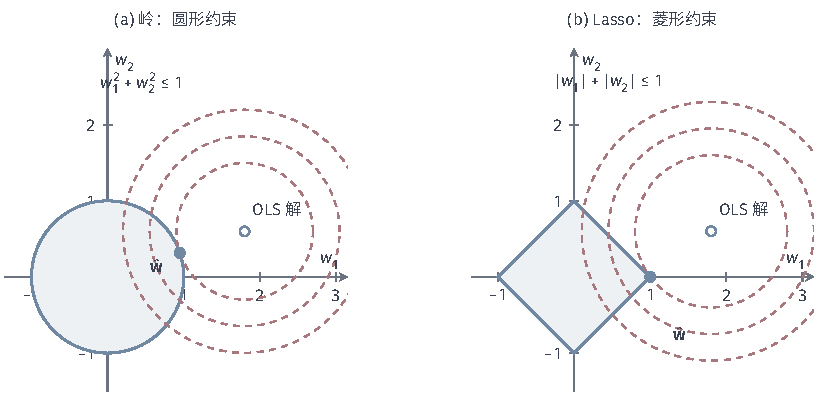
\includegraphics[width=138.649mm]{figures/04-classic-models/00-shared/tikz/regression-regularization-geometry/figure.pdf}
  \caption{岭与Lasso的约束几何。构造损失为$J(\bm{w})=\lVert\bm{w}-(1.8,0.6)^{\top}\rVert_2^2/2$，虚线为等损失线，浅色区域为可行域，空心点为OLS解，实心点为约束最优解。左图解为$(1.8,0.6)^{\top}/\sqrt{3.6}$，右图解为$(1,0)^{\top}$。两图都取单位约束半径以比较形状，不表示相同的惩罚强度；Lasso也并非总在尖点取到最优解。}
  \label{fig:regression-regularization-geometry}
\end{figure*}

岭惩罚沿设计矩阵的谱方向收缩系数，一般设计下各原始坐标受到的相对收缩可以不同，下面将给出相应分解。惩罚的概率解释同样依赖归一化：高斯似然下，高斯先验对应二次惩罚，各系数独立的拉普拉斯先验（Laplace prior）对应一范数惩罚，但先验尺度与$\lambda$的对应关系还包含$n$和噪声方差。

\subsubsection{参数学习}
\label{sec:regression-regularization-learning}

岭回归仍有直接求解与迭代求解两条路线。先把平方损失与二次惩罚相加，再对系数求导。令梯度$\bm X^\top(\bm X\bm w-\bm y)/n+\lambda\bm w$为零，便得到一个在OLS正规方程上增加$n\lambda\bm I$的线性系统；其解为
\begin{equation}
  \widehat{\bm{w}}_{\lambda}
  =(\bm{X}^{\top}\bm{X}+n\lambda\bm{I})^{-1}\bm{X}^{\top}\bm{y},
  \qquad\lambda>0.
  \label{eq:regression-ridge-solution}
\end{equation}
任意非零$\bm{v}$满足$\bm{v}^{\top}(\bm{X}^{\top}\bm{X}+n\lambda\bm{I})\bm{v}=\lVert\bm{X}\bm{v}\rVert_2^2+n\lambda\lVert\bm{v}\rVert_2^2>0$，所以即使设计秩亏，斜率解也唯一。若$\gamma_{\max},\gamma_{\min}$是$\bm{X}^{\top}\bm{X}$的极端特征值，正则化后该矩阵的条件数为$(\gamma_{\max}+n\lambda)/(\gamma_{\min}+n\lambda)$；比较对象是正规方程矩阵，而非$\bm{X}$本身的条件数。

取$\bm{X}=\bm{U}_r\bm{D}_r\bm{V}_r^{\top}$，正奇异值为$s_j$，则
\begin{equation}
  \bm{X}\widehat{\bm{w}}_{\lambda}
  =\sum_{j=1}^{r}\frac{s_j^2}{s_j^2+n\lambda}
       \bm{u}_j\bm{u}_j^{\top}\bm{y}.
  \label{eq:regression-ridge-spectral}
\end{equation}
OLS保留列空间中的全部投影，岭回归则按$s_j^2/(s_j^2+n\lambda)$保留各方向，小奇异值方向受到更强收缩。这是稳定性改善的来源，也说明惩罚会同时压低这些方向上的真实信号。

这一分解可由前面介绍的SVD直接算出。沿$\bm v_j$方向，$\bm X^\top\bm X+n\lambda\bm I$的特征值为$s_j^2+n\lambda$，而$\bm X^\top\bm y$在该方向的分量为$s_j\bm u_j^\top\bm y$。因此岭系数在此方向等于$s_j\bm u_j^\top\bm y/(s_j^2+n\lambda)$；再乘$\bm X$产生训练预测时，多出一个$s_j$，就得到式\eqref{eq:regression-ridge-spectral}的因子。$\bm X$零空间中的右端分量为零，岭解在这些方向也取零。这里的$\bm u_j$仍是$n$维训练预测方向，并不是原始输入坐标。

Lasso的目标记为$F(\bm{w})$。由于$\lambda>0$时$F(\bm{w})\geq\lambda\lVert\bm{w}\rVert_1$，连续目标至少取得一个最小值；参数解未必唯一。要理解零系数为何可能最优，可以先固定其他坐标。令$\bm{r}_{-j}=\bm{y}-\sum_{k\ne j}\bm{X}_{:,k}w_k$，$a_j=\lVert\bm{X}_{:,j}\rVert_2^2/n$、$c_j=\bm{X}_{:,j}^{\top}\bm{r}_{-j}/n$，略去常数后的单坐标目标为
\[
  q_j(w_j)=\frac{a_j}{2}w_j^2-c_jw_j+\lambda|w_j|.
\]
在零点左侧，绝对值项的斜率为$-\lambda$；右侧则为$\lambda$。因此零点的左右导数分别为
\[
  q'_{j,-}(0)=-c_j-\lambda,\qquad
  q'_{j,+}(0)=-c_j+\lambda.
\]
这个目标是凸函数，零点最优恰好要求左导数不大于零、右导数不小于零，即$|c_j|\leq\lambda$。此时无论向哪一侧离开零点，目标都不会降低；损失项在零点的导数$-c_j$却不必为零。

刚才的零系数虽然已经最优，损失项的导数却不一定为零，而绝对值惩罚在零点又没有普通导数。因此，OLS使用的“总梯度等于零”不能直接检验这个解。我们需要一种允许惩罚在零点提供一段斜率、并检验这些斜率能否抵消损失导数的条件。

\term{次梯度}（subgradient）用位于凸函数下方的支持直线描述这些可用斜率。对一维凸函数$f$，若斜率$s$满足$f(v)\geq f(u)+s(v-u)$对所有$v$成立，它就是$f$在$u$处的一个次梯度：经过该点、斜率为$s$的直线始终位于函数图像下方。所有这样的斜率组成次梯度集合$\partial f(u)$；可导时集合只有导数一个元素，而$|u|$在零点允许$[-1,1]$中的全部斜率。

凸函数的最优性因而可统一表为$0\in\partial f(u)$。对Lasso，损失梯度加上惩罚次梯度为零，得到充要最优性条件
\begin{equation}
  \frac{\bm{X}^{\top}(\bm{y}-\bm{X}\widehat{\bm{w}})}{n}
  =\lambda\bm{z},\qquad
  z_j\in
  \begin{cases}
    \{\operatorname{sign}(\widehat w_j)\},&\widehat w_j\ne0,\\
    [-1,1],&\widehat w_j=0.
  \end{cases}
  \label{eq:regression-lasso-kkt}
\end{equation}
其中非零坐标对应的绝对值导数为符号函数，零坐标则允许整个区间来抵消损失梯度。沿用上述$a_j,c_j$，在正、负半轴求导，并在零点检验$|c_j|\leq\lambda$，得到坐标更新
\begin{equation}
  w_j\leftarrow\frac{\mathcal{S}_{\lambda}(c_j)}{a_j},
  \qquad
  \mathcal{S}_{\lambda}(c)=\operatorname{sign}(c)(|c|-\lambda)_+.
  \label{eq:regression-soft-threshold}
\end{equation}
这里$a_j>0$，零列直接取零系数。\term{软阈值}（soft thresholding）把阈值内的量置零，将其余量向零移动$\lambda$。例如正交标准化设计下，OLS系数$(0.12,1.40)$在$\lambda=0.20$时变为$(0,1.20)$；相关设计则需反复更新部分残差，不能直接阈值化OLS系数。循环坐标下降可用式\eqref{eq:regression-lasso-kkt}的违反程度作为停止依据。

回到前面的正交例子，此时$a_j=1$，其他列与第$j$列正交，因而$c_j=\bm X_{:,j}^\top\bm y/n$不随其他坐标的更新改变，恰好就是该坐标的OLS系数。这说明何以能够一次对OLS系数应用阈值。一般相关设计没有这个消去交叉项的条件，所以每次更改一个坐标后，其余坐标的部分残差也必须跟着更新。

弹性网的坐标更新为$\mathcal{S}_{\lambda_1}(c_j)/(a_j+\lambda_2)$。

组惩罚需要对整段系数共同作取舍。记光滑数据项为$g(\bm w)=\lVert\bm y-\bm X\bm w\rVert_2^2/(2n)$，把惩罚另记为$\operatorname{pen}(\bm w)$。数据项处处可微，一范数与组范数却在零点有尖点，不能简单套用“求梯度再沿负方向走一步”；而且组Lasso的最小单位是一整组系数，逐坐标更新无法判断整组是否该一起置零。近端梯度（proximal gradient）专为“光滑项＋带尖角的凸惩罚”这种组合设计：先用一条简单的二次函数在当前点附近从上方近似光滑的数据项，把“向数据更吻合的方向走一步”与“缩小惩罚”合并成一个通常有闭式答案的子问题。非零设计下，令$L=\lVert\bm X^\top\bm X/n\rVert_2$，取$0<t\leq1/L$，则
\[
 \begin{aligned}
 g(\bm u)&\leq g(\bm w)+\nabla g(\bm w)^\top(\bm u-\bm w)\\
 &\qquad+\frac{1}{2t}\lVert\bm u-\bm w\rVert_2^2.
 \end{aligned}
\]
把右侧与原惩罚相加，再对二次项配方，就得到$\min_{\bm u}\lVert\bm u-\bm v\rVert_2^2/2+t\operatorname{pen}(\bm u)$，其中$\bm v=\bm w-t\nabla g(\bm w)$。这个子问题在“靠近数据项的梯度步”与“减小惩罚”之间作取舍；由于原惩罚没有被求导，零点的尖角及选择作用仍然保留。不重叠组的平方距离与惩罚都能按组相加，所以这个子问题可以分组求解。

组惩罚则可用近端梯度：先令$\bm{v}=\bm{w}-t\bm{X}^{\top}(\bm{X}\bm{w}-\bm{y})/n$，再逐组计算
\begin{equation}
  \bm{w}_{A_g}^{+}
  =
  \begin{cases}
    \bm{0},&\lVert\bm{v}_{A_g}\rVert_2\leq t\lambda\omega_g,\\
    \left(1-\dfrac{t\lambda\omega_g}{\lVert\bm{v}_{A_g}\rVert_2}\right)
      \bm{v}_{A_g},&\text{其他情形}.
  \end{cases}
  \label{eq:regression-group-prox}
\end{equation}
该式求解的是$\min_{\bm{u}}\lVert\bm{u}-\bm{v}_{A_g}\rVert_2^2/2+t\lambda\omega_g\lVert\bm{u}\rVert_2$：固定$\lVert\bm{u}\rVert_2$时，同向选择使平方距离最小，剩下的一维非负半轴问题给出径向阈值。该闭式解针对欧氏距离构成的近端子问题；一般设计的块坐标子问题还包含组内设计的曲率，需要据此求解。对非零设计，取$0<t\leq1/\lVert\bm{X}^{\top}\bm{X}/n\rVert_2$可保证凸近端梯度法的目标收敛性质。

具体地，当$\bm v_{A_g}\ne\bm0$时，把同向候选写成$\bm u=r\bm v_{A_g}/\lVert\bm v_{A_g}\rVert_2$，其中$r\geq0$。要最小化的标量目标就是
\[
 \frac12(r-\lVert\bm v_{A_g}\rVert_2)^2
       +t\lambda\omega_g r,\qquad r\geq0.
\]
其内部驻点为$r=\lVert\bm v_{A_g}\rVert_2-t\lambda\omega_g$；若这个值为负，约束最小点就在$r=0$。合起来即$r=(\lVert\bm v_{A_g}\rVert_2-t\lambda\omega_g)_+$，代回同向候选就得到组阈值公式。$\bm v_{A_g}=\bm0$时直接取零，不需要作除法。

沿$\lambda$网格使用前一个解热启动，可以减少重复计算。LARS的Lasso修正版利用分段线性路径求解一范数惩罚问题，但这一性质不直接推广到一般Group Lasso。超参数通常由交叉验证选择；中心化、标准化与变量选择都必须在每个训练折内完成。跨软件比较超参数时，应先将平方损失与惩罚换算到相同的系数约定\scite{hastie2009}。

这里的LARS指最小角回归（least angle regression）算法。理解上述路径只需抓住一段局部机制：在活跃列线性独立、非零坐标及其符号保持不变的一段上，Lasso最优性方程是关于这些系数的线性系统，右端随$\lambda$作线性变化，所以解也随$\lambda$作线性变化。变量进入、退出或符号改变时，进入另一段；LARS的修正版据此追踪路径。这项说明不把所有组范数惩罚都视为同样的折线。

\subsubsection{收缩的收益与变量选择的边界}
\label{sec:regression-regularization-theory}
\label{sec:regression-elastic-net}
\label{sec:regression-group-lasso}

正则化没有自动增加特征中缺少的函数。有限惩罚改变的是从原有系数中怎样取舍；硬约束才会直接排除范围外的候选。岭的谱因子显示，小奇异值方向的噪声与真实信号都会被压低，所以稳定系数要付出偏差代价。

正则化用偏差换方差，值得把这两个词讲具体。模型是在一个有限训练集上训练出来的：如果同样的数据生成过程重新抽样，得到一批新的训练记录，再用完全相同的方法训练，新模型的预测通常会和旧模型略有不同。所谓方差，就是预测在这种“换一批训练集”的重复实验中围绕自身平均值的摆动；所谓偏差，是这些预测的平均值与真实条件均值之间的固定差距。固定未来输入$\bm x$，设其响应均值为$m(\bm x)$，未来噪声独立于训练记录且方差有限。把由不同训练集得到的预测再取平均，平方误差便分解为
\[
 \begin{aligned}
 \mathbb E[(Y_\star-\widehat f(\bm x))^2\mid\bm x]
 &=\operatorname{Var}(Y_\star\mid\bm x)\\
 &\quad+[\mathbb E\widehat f(\bm x)-m(\bm x)]^2\\
 &\quad+\operatorname{Var}(\widehat f(\bm x)).
 \end{aligned}
\]
把误差拆成未来噪声、平均预测偏离真实均值、以及预测围绕其平均的波动，展开平方后交叉项的期望为零，就得到这三项。惩罚可能降低最后一项，同时增大中间一项；是否有益要比较两者之和。图\ref{fig:regression-bias-variance-noise}给出这种取舍的示意，不是对任意数据的性能排序。

\begin{figure}[htbp]
  \centering
  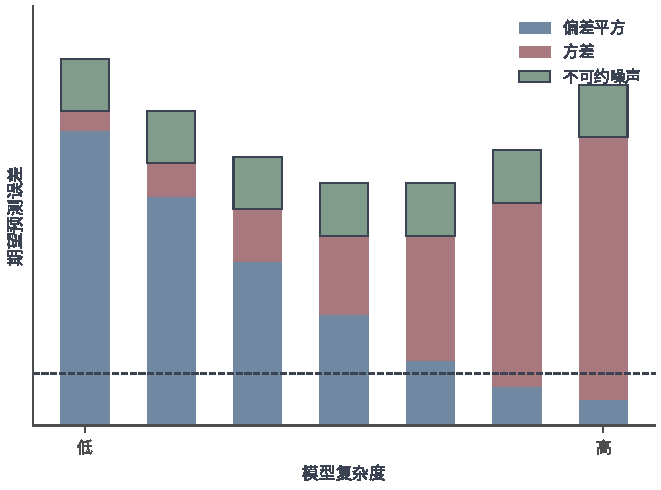
\includegraphics[width=105.412mm]{figures/04-classic-models/00-shared/matplotlib/regression-bias-variance-noise/figure.pdf}
  \caption{模型复杂度变化时的偏差—方差—噪声分解示意。柱高是教学构造的相对量，不来自实验：复杂度增加时偏差平方下降、估计方差上升，不可约噪声保持不变。总误差由三部分共同决定，因此“模型更复杂”与“误差更小”都不是无条件结论。}
  \label{fig:regression-bias-variance-noise}
\end{figure}

变量选择还要区分“预测准确”与“识别真实变量”。两个高度相关变量可能互相替代，预测仍然接近，选中哪个却会随样本变化。弹性网的正二次惩罚使解唯一；两列完全相同时，交换系数不改变目标，唯一性便要求它们相等。组Lasso则按预定组共同取舍，不能据此保证组内每个坐标都非零。若希望同时选择组与组内坐标，可以在组惩罚之外再加$\lambda_1\lVert\bm w\rVert_1$，得到\term{稀疏组Lasso}（sparse group Lasso）；对互不重叠的组，学习时先对梯度步作阈值$t\lambda_1$的坐标软阈值，再按组作阈值$t\lambda\omega_g$的径向阈值，正则强度仍由训练内验证选择。

\subsubsection{成分回归：PCR与PLS}

\label{sec:regression-component-regression}

处理共线性的另一条路线不是给系数加惩罚，而是先对输入本身做一次“改换坐标系”的预处理：把众多彼此相关的原始变量合成为少数几个互不相关的综合指标（成分），再在这些成分上做回归。由于成分数量少且相互正交，在它们上面估计系数就避开了“两列几乎相同、系数无法分辨”的问题；代价是必须决定保留多少、保留哪些成分。\term{主成分回归}（principal component regression, PCR）保留若干主成分，在这些正交方向上拟合，等价于对选中方向完全保留、对其余方向硬截断。第\ref{sec:dim-pca}节从无监督表示的角度推导主成分分析（PCA）：PCA与PCR共享由输入方差确定的主成分基，但PCA按方差保留与重构误差评价表示，PCR还要用响应检验这些成分是否有利于预测。与式\eqref{eq:regression-ridge-spectral}的连续收缩相比，PCR的取舍更直接，但输入方差小不意味着对响应不重要。\term{偏最小二乘回归}（partial least squares regression, PLS）在构造成分时同时利用输入与响应的关系，因而属于监督降维；它有不同的具体算法，不能笼统理解为收缩因子必在$0$和$1$之间的岭回归。

以一种常见的单响应线性PLS构造为例，先将输入与响应中心化，把总体随机输入向量另记为$\bm Z=(X_1,\ldots,X_d)^\top$。在单位系数方向$\lVert\bm a\rVert_2=1$中寻找成分$T=\bm a^\top\bm Z$，使$\operatorname{Cov}(T,Y)^2$最大；训练时用样本协方差代替总体协方差，仍由设计矩阵$\bm X$得到样本成分向量$\bm t=\bm X\bm a$。单位长度约束防止仅靠放大系数无限增大协方差，使用响应协方差则使方向选择面向预测。后续成分在已解释部分移除后继续提取信息，并满足所用算法的正交要求；具体消去方式随PLS算法而异。

例如教学构造中，$X_1,X_2$独立、方差分别为$100$与$1$，响应为$Y=X_2$。不额外标准化时，PCA的第一主成分为$X_1$；只保留这一成分做PCR会丢掉全部响应信号。PLS构造成分时利用输入与响应的关系，在这个例子中可以识别$X_2$与$Y$的关联，而不只按输入方差决定取舍。成分数同样需要在训练折内选择。

刚才的教学分布给出$\operatorname{Cov}(X_1,Y)=0$、$\operatorname{Cov}(X_2,Y)=1$，所以$\operatorname{Cov}(a_1X_1+a_2X_2,Y)=a_2$。在$a_1^2+a_2^2=1$下，协方差平方在$a_1=0$、$|a_2|=1$时最大，即选中$X_2$方向；PCA的方差准则则选中$X_1$方向。这个计算只比较两种方法怎样选第一成分，不声称有限样本总能准确识别信号，也不替代成分数的训练折内选择。

选出成分还没有完成回归。把训练得到的线性变换记为$\bm R\in\mathbb R^{d\times m}$，成分设计为$\bm T=\bm X\bm R$；PCR取选中的主成分方向，PLS则使用其训练算法给出的成分变换。接着拟合
\[
 \begin{aligned}
 \widehat{\bm\gamma}&\in\argmin_{\bm\gamma}
       \|\bm y-\bm T\bm\gamma\|_2^2,\\
 \widehat f(\bm x)&=\bar y+
       (\bm x-\bar{\bm x})^\top\bm R\widehat{\bm\gamma}.
 \end{aligned}
\]
这里$\bm X,\bm y$已中心化，$\bar{\bm x},\bar y$来自该训练折；若还做标准化，新输入也要用同一尺度。使用PLS时，新输入必须经过训练中固定下来的同一套成分变换，不能重新按新响应选择方向。最后由验证比较成分数，既不能只保留方差最大的方向就结束，也不能只计算协方差方向而省略响应系数的学习\scite{hastie2009}。

\label{sec:regression-regularization-summary}
惩罚约束原坐标中的系数，PCR与PLS先改变回归使用的方向；两条路线都需在验证中决定保留多少信息。尺度处理、成分提取与变量选择必须跟随每个训练折重新完成。

\subsection{分位数回归（Quantile Regression）}
\label{sec:regression-quantiles}

预算制定者关心的是实际支出超过预算的概率，单个条件均值无法回答这个问题。假设同类任务的支出以$80\%$概率为$100$，以$20\%$概率为$200$。平均支出是$120$，照此准备预算仍有$20\%$概率超支；如果要求至少$90\%$的支出不超过预算，这个例子中应把阈值提高到$200$。两种预测使用同一响应分布，差别来自需要完成的决策。\term{分位数回归}（quantile regression）用非对称残差损失估计给定输入后的指定分位数；例如$0.9$分位数提供一个使响应至少有$90\%$概率不超过它的条件阈值。Koenker与Bassett在1978年系统提出回归分位数，将回归目标从条件均值扩展到条件分布的不同位置。这一区分源于决策目标，无需先假定误差对称或同方差\scite{koenker1978quantiles}。

\subsubsection{模型结构}

预算阈值低估时产生超支，高估时则预留过多；两种偏差的代价可以不同，而平方损失对高估和低估一视同仁，无法表达这种不对称。要估计某个分位数，就要让落在阈值两侧的误差按不同的权重计分：估低了（实际值高于预测）更接近我们想避免的超支，就给更高的权重。给定$0<\tau<1$，\term{分位数损失}（pinball loss）用$\tau$和$1-\tau$分别给正、负残差计分：
\begin{equation}
  \rho_\tau(r)=
  \begin{cases}
    \tau r,&r\geq0,\\
    (1-\tau)(-r),&r<0.
  \end{cases}
  \label{eq:regression-pinball}
\end{equation}
残差仍取$r=y-\widehat y$，所以较大的$\tau$更重地惩罚低估。线性分位数回归最小化$\sum_i\rho_\tau(y_i-\bm\phi(\bm x_i)^\top\bm w)$。要说明这种非对称计分为什么选择分位数，可以先只预测一个常数$a$。对前面固定的$0<\tau<1$，假设$\mathbb E|Y|<\infty$，记响应分布函数为$F_Y$，期望损失为$Q(a)=\mathbb E[\rho_\tau(Y-a)]$。

我们比较把$a$提高一点以后，损失怎样改变。若$Y<a$，这次调整加重高估，单位变化的代价为$1-\tau$；若$Y>a$，调整减轻低估，单位变化的损失减少$\tau$。当响应恰好等于$a$时，向左、向右的变化率不同，所以要分别计算单侧导数。单条损失的变化率始终有界，因而可以在期望内取相应单侧极限，得到
\begin{equation}
 \begin{aligned}
  Q'_-(a)&=(1-\tau)\mathbb P(Y<a)
            -\tau\mathbb P(Y\geq a)\\
          &=F_Y(a-)-\tau,\\
  Q'_+(a)&=(1-\tau)\mathbb P(Y\leq a)
            -\tau\mathbb P(Y>a)\\
          &=F_Y(a)-\tau.
 \end{aligned}
 \label{eq:regression-pinball-one-sided}
\end{equation}
$Q$是凸函数，最优点要求左导数不大于零、右导数不小于零；因此，它的全部最小点恰好满足
\[
 F_Y(a-)\leq\tau\leq F_Y(a),
 \qquad F_Y(a-)=\mathbb P(Y<a).
\]
这两条不等式同时处理了响应在某一点具有正概率的情形，以及分布函数在一段区间上保持不变的情形；它们保留了可能不唯一的最优点集合。以刚才两种支出为例，$\tau=0.9$、$a=200$时，左、右导数分别为$0.8-0.9=-0.1$和$1-0.9=0.1$，向任一侧移动都不能降低期望损失。若改取$\tau=0.8$，则$[100,200]$中的每个阈值都满足上述条件，整个区间的期望损失相同。

将分布换成给定输入的条件分布，便得到条件分位数；换成经验分布，便得到样本分位数。$\tau=1/2$时损失为$|r|/2$，对应中位数。在线性模型受到限制时，只有正确指定等条件下才能精确表示真实条件分位数，一般得到该函数类中的最佳损失逼近。

图\ref{fig:regression-quantile-objective}用只有截距的模型展示这一选择：同一组响应，在不同$\tau$下对应不同的最优阈值。较大的$\tau$给低估更高的代价，最优预测也向较高的响应移动；分位数回归把这个目标进一步应用到每个输入的条件分布。

\begin{figure*}[htbp]
  \centering
  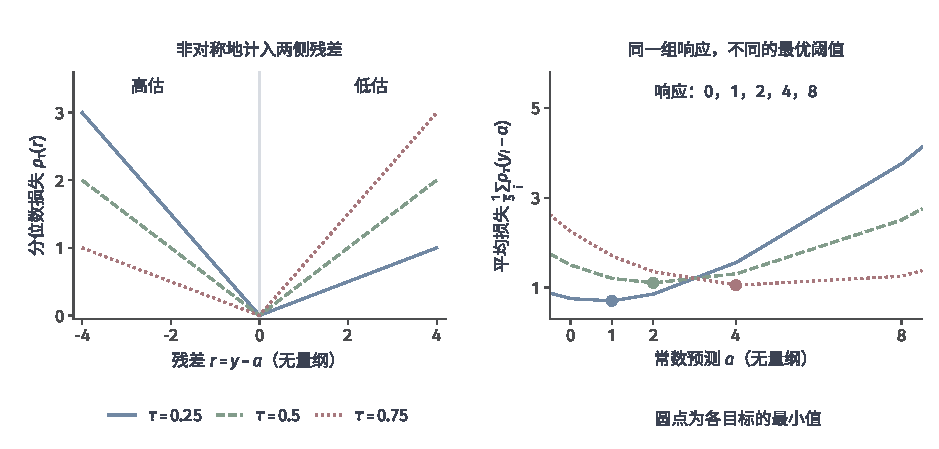
\includegraphics[width=159mm]{figures/04-classic-models/00-shared/matplotlib/regression-quantile-objective/figure.pdf}
  \caption{分位数损失怎样改变学习目标。左图中，正残差表示低估、负残差表示高估；$\tau$越大，低估一单位的代价越高。右图对固定响应$0,1,2,4,8$比较三个平均损失目标，其唯一最小点分别为$1,2,4$，对应经验分布的$0.25,0.5,0.75$分位数。数值均为无量纲教学构造，圆点表示最小值。}
  \label{fig:regression-quantile-objective}
\end{figure*}

\subsubsection{参数学习}

分位数损失在零残差处不可微，因而不宜像OLS那样直接解梯度为零的方程。我们可以把每个残差拆成正、负两部分，分别按$\tau$和$1-\tau$计分。引入非负变量$\bm u,\bm v\in\mathbb R^n$，将残差写成$\bm y-\bm X\bm w=\bm u-\bm v$，便得到线性规划
\begin{equation}
  \begin{aligned}
    \min_{\bm{w},\bm{u},\bm{v}}\quad&
      \tau\bm{1}^{\top}\bm{u}+(1-\tau)\bm{1}^{\top}\bm{v},\\
    \text{满足}\quad&
      \bm{y}-\bm{X}\bm{w}=\bm{u}-\bm{v},
      \quad\bm{u}\geq\bm{0},\ \bm{v}\geq\bm{0}.
  \end{aligned}
  \label{eq:regression-quantile-lp}
\end{equation}
若某个$u_i,v_i$同时为正，同时减小二者保持约束不变且严格降低目标，因此最优时二者不会同时为正，线性规划与原损失等价。可采用单纯形法、内点法或适合数据规模的非光滑凸优化算法；这些算法分别利用线性规划结构或直接处理非光滑凸目标。

有限样本的线性规划有可行解，目标下有界于零，因此能取得最优值，但系数和分位数都可能不唯一。停止时可比较原始与对偶可行目标的间隙，而不能直接检查普通梯度是否为零。极端分位数由较少尾部观测支持，需要特别检查验证损失与经验超越率。

\subsubsection{稀疏分位数与有序分位数}

\label{sec:regression-quantile-sparsity}

变量很多、尾部观测有限时，估计每个变量的作用容易受个别记录影响。可在平均分位数损失之外增加$\lambda\lVert\bm w\rVert_1$，使部分系数可以取零。把系数也拆成正、负两部分，仍可将这一目标写成线性规划。这与Lasso使用相同的系数约束，却保留分位数损失规定的预测对象；$\lambda$应按验证分位数损失选择，不能只凭平方误差判断。

\label{sec:regression-quantile-ordering}

若分别估计预算的中位数和较高分位数，两条曲线可能在某些输入处交叉，使较高分位数反而更低。可以同时拟合多个$\tau$，在预先指定的输入集合$\mathcal X_0$上加入顺序约束：对$\tau_1<\tau_2$，要求$\bm\phi(\bm x)^\top\bm w_{\tau_1}\leq\bm\phi(\bm x)^\top\bm w_{\tau_2}$，$\bm x\in\mathcal X_0$。对有限$\mathcal X_0$，这些是线性约束，可以和各分位数的残差分解一起求解。它们只保证指定输入处的顺序；要保证整个输入域不交叉，还需对该域施加足够的约束。联合拟合增加系数和约束数量，但避免了在各分位数之间分别选择互不协调的预测。

多个分位数能描述分布的不同位置，但有限网格不等于完整条件分布；由它们组成的预测区间仍需单独评价响应覆盖率与宽度。

\subsection{支持向量回归（SVR）}
\label{sec:regression-svr}

有些任务并不要求把每一个小偏差都继续压低，小到一定程度的误差在实际决策中与完全正确没有区别。例如，假设测量任务把$0.05$单位以内的误差都视为可接受；真实响应为$2.00$时，预测$1.98$已在容忍范围内，而预测$1.80$超出范围$0.15$。平方损失仍会区分带内的细小误差（$0.02$和$0.04$受到不同惩罚），分位数损失则对每个非零残差计分。另一种选择是让容忍范围内的损失直接为零，只对超出部分计分。\term{支持向量回归}（support vector regression, SVR）将这种损失与二次正则化结合，得到一个由训练样本加权表示的预测函数。部分样本的权重可以为零，核化以后只需保留非零权重对应的样本来计算预测。这是样本展开的稀疏性，与Lasso选择输入变量的稀疏性不同\scite{smola2004svr}。

\subsubsection{模型结构}

设$\epsilon\geq0$，定义\term{$\epsilon$不敏感损失}（$\epsilon$-insensitive loss）为$L_\epsilon(r)=(|r|-\epsilon)_+$。它把$\pm\epsilon$之间的残差视为可容忍误差，超出部分线性计入损失。线性SVR单独保留不受惩罚的截距$b$，目标为
\begin{equation}
  \min_{\bm{w},b}\;
    \frac12\lVert\bm{w}\rVert_2^2+
    C\sum_{i=1}^{n}L_\epsilon(y_i-\bm{w}^{\top}\bm{x}_i-b),
    \qquad C>0.
  \label{eq:regression-svr-objective}
\end{equation}
除以$nC$，可知它与“平均损失$+\lambda\lVert\bm{w}\rVert_2^2/2$”在$\lambda=1/(nC)$时等价。$C$越大，训练误差在目标中的相对权重越大；$\epsilon$则具有响应的单位，规定不计损失的范围。

图\ref{fig:regression-svr-objective}把损失画回响应坐标：围绕候选函数的带内偏差都不计分，带外残差只有超过边缘的部分计分。学习时还要加入斜率或核函数范数的惩罚，所以扩大容忍带、减小带外误差与选择较平缓的函数，是目标中的不同调节。

\begin{figure*}[htbp]
  \centering
  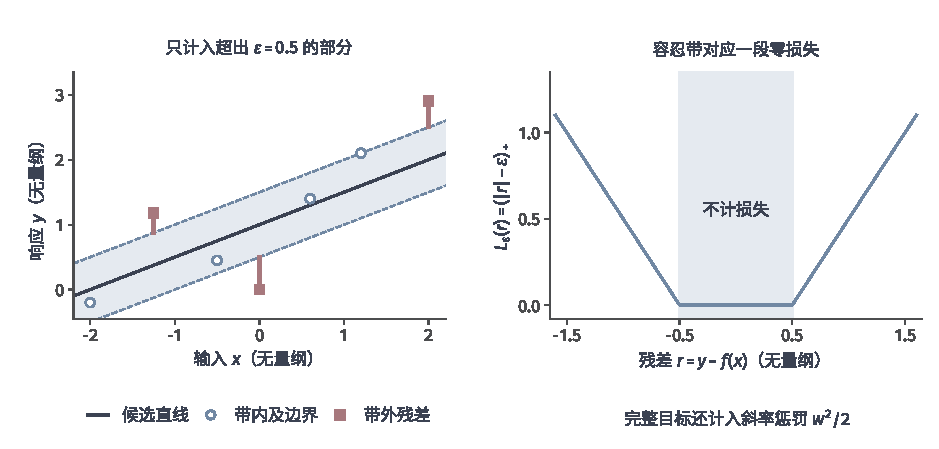
\includegraphics[width=159mm]{figures/04-classic-models/00-shared/matplotlib/regression-svr-objective/figure.pdf}
  \caption{SVR的容忍带与带外损失。左图取候选$f(x)=1+x/2$、$\epsilon=0.5$，圆点位于带内或边界，方点位于带外；红色竖段只标记超出带边缘的部分。右图将同一规则写成残差损失，带内损失为零、带外线性增长。构造样本的损失之和为$1.2$，斜率惩罚为$0.125$，因此该候选的完整目标为$0.125+1.2C$；图中不假定它是最优解。}
  \label{fig:regression-svr-objective}
\end{figure*}

损失在容忍带边缘不可微，直接用普通梯度求解并不方便。我们可以用两个非负量$\xi_i^+,\xi_i^-\geq0$，分别记录残差从两侧超出容忍带的部分；损失于是成为它们的和，而预测条件变成线性约束。这个等价形式也便于推导只依赖样本内积的对偶问题：
\begin{equation}
  \begin{aligned}
    \min_{\bm{w},b,\bm{\xi}^+,\bm{\xi}^-}\quad&
       \tfrac12\lVert\bm{w}\rVert_2^2+C\sum_i(\xi_i^++\xi_i^-),\\
    \text{满足}\quad&
       y_i-\bm{w}^{\top}\bm{x}_i-b\leq\epsilon+\xi_i^+,\\
      &\bm{w}^{\top}\bm{x}_i+b-y_i\leq\epsilon+\xi_i^-,\\
      &\xi_i^+,\xi_i^-\geq0,\qquad i=1,\ldots,n.
  \end{aligned}
  \label{eq:regression-svr-primal}
\end{equation}
固定预测时，由$C>0$可知最优松弛量恰为超出带宽的部分。$\epsilon=0$对应带二次惩罚的绝对损失回归。对固定有限数据，若$\epsilon\geq(\max_i y_i-\min_i y_i)/2$，则$\bm{w}=\bm{0}$和某个常数$b$已能使全部样本进入容忍带，目标取得零值。截距在此时可能不唯一。

\subsubsection{参数学习}

原问题是在可行参数中寻找最小目标值，为什么下面会出现一个最大化问题？把各不等式写成“左边不大于零”，分别乘以非负的拉格朗日乘子并加到目标中，就得到拉格朗日函数。在任一可行点，这些附加项都不大于零；固定乘子，再对全部原始变量取下确界，便得到原问题最优值的一个下界。选择乘子把这个下界尽量抬高，就是\term{对偶}（dual）最大化。乘子在这里用于构造下界；若最佳下界等于原问题的最小值，就称为\term{强对偶}（strong duality）。

下面用凸优化条件判断这一对应何时成立。为方便首次接触这些名词的读者，先用一句话说明它们各自扮演的角色：拉格朗日乘子可以理解为每条约束“被违反的价格”，违反越严重、价格越高，于是原问题转化为在这些价格下的权衡；Slater条件是一个保证“抬高下界”这条路能够恰好达到原问题最优值的正则性条件，它在当前凸问题中用于建立强对偶；KKT条件则是最优解必须同时满足的一份清单，把原始可行性、对偶可行性、驻点条件和互补松弛放在同一组方程中，其中互补松弛要求“约束没有被绷紧时，它的价格必须为零”，即乘子与对应约束余量的乘积为零。在凸问题满足Slater条件时，满足这份清单对最优性既必要又充分；分类SVM中的对应条件见式\eqref{eq:classification-svm-hard-kkt}。

为前两组约束引入乘子$\alpha_i^+,\alpha_i^-\geq0$，为松弛量非负约束引入$\mu_i^+,\mu_i^-\geq0$。令$r_i=y_i-\bm{w}^{\top}\bm{x}_i-b$，拉格朗日函数为
\[
  \begin{aligned}
    \mathcal{L}={}&\tfrac12\lVert\bm{w}\rVert_2^2
       +C\sum_i(\xi_i^++\xi_i^-)
       +\sum_i\alpha_i^+(r_i-\epsilon-\xi_i^+)\\
       &+\sum_i\alpha_i^-(-r_i-\epsilon-\xi_i^-)
       -\sum_i(\mu_i^+\xi_i^++\mu_i^-\xi_i^-).
  \end{aligned}
\]
分别对$\bm{w},b,\xi_i^\pm$求导，得到
\[
  \bm{w}=\sum_i(\alpha_i^+-\alpha_i^-)\bm{x}_i,\qquad
  \sum_i(\alpha_i^+-\alpha_i^-)=0,\qquad
  C-\alpha_i^\pm-\mu_i^\pm=0.
\]
最后一式给出$0\leq\alpha_i^\pm\leq C$。记$\beta_i=\alpha_i^+-\alpha_i^-$，消去原始变量后，对偶问题为
\begin{equation}
  \begin{aligned}
    \max_{\bm{\alpha}^+,\bm{\alpha}^-}\quad&
       -\tfrac12\sum_{i,j}\beta_i\beta_j\bm{x}_i^{\top}\bm{x}_j
       -\epsilon\sum_i(\alpha_i^++\alpha_i^-)
       +\sum_i y_i\beta_i,\\
    \text{满足}\quad&
       \sum_i\beta_i=0,\qquad 0\leq\alpha_i^\pm\leq C.
  \end{aligned}
  \label{eq:regression-svr-dual}
\end{equation}
原始问题凸，选择足够大的正松弛量即可严格满足不等式，因此满足Slater条件，强对偶成立。对偶是带盒约束与一个线性等式约束的凸二次规划的最大化写法，可通过分解算法逐步更新少量变量；每次更新应保持等式约束，并以最优性残差作为停止依据。

得到乘子后，若$0<\alpha_i^+<C$，互补松弛给出$r_i=\epsilon$，所以$b=y_i-\bm{w}^{\top}\bm{x}_i-\epsilon$；若$0<\alpha_i^-<C$，则$b=y_i-\bm{w}^{\top}\bm{x}_i+\epsilon$。可对多个此类样本的截距估计取平均以减小数值误差。若没有内点乘子，应根据全部KKT不等式求可行截距区间，不能假设总能找到一个严格介于$0$与$C$之间的乘子。

\subsubsection{核SVR与支持样本}
\label{sec:regression-svr-theory}
\label{sec:regression-rkhs-foundations}
\label{sec:regression-kernel-svr}

原始特征不足以表达弯曲关系时，可以保留同一个容忍带损失，只把对偶中的内积换成合法核$K(\bm x_i,\bm x_j)$。这等于在核所表示的特征空间中惩罚权重长度，预测变为
\begin{equation}
 f(\bm x)=\sum_{i=1}^n\beta_iK(\bm x_i,\bm x)+b.
 \label{eq:regression-kernel-svr-prediction}
\end{equation}
核的合法性与常用形式见第\ref{sec:classic-overview-kernel-validity}节和第\ref{sec:classic-overview-common-kernels}节。训练仍解式\eqref{eq:regression-svr-dual}的盒约束二次规划，只需更换Gram矩阵；核、$C$与$\epsilon$则一起由训练内验证选择。

为说明这里惩罚的对象，把$K(\bm x_i,\cdot)$看成关于新输入的函数，称为核截面（kernel section）。若$h=\sum_i a_iK(\bm x_i,\cdot)$、$v=\sum_j c_jK(\bm z_j,\cdot)$，核定义的内积和范数满足
\begin{equation}
 \begin{aligned}
 \langle h,v\rangle_{\mathcal H_K}
 &=\sum_{i,j}a_ic_jK(\bm x_i,\bm z_j),\\
 \|h\|_{\mathcal H_K}^2&=\bm a^\top\bm K\bm a.
 \end{aligned}
 \label{eq:regression-rkhs-inner-product}
\end{equation}
相差零范数的表示视为同一函数，并纳入范数极限后，就得到\term{再生核Hilbert空间}（reproducing kernel Hilbert space, RKHS），记为$\mathcal H_K$。它把特征空间中的长度写成可以由核值计算的函数范数，而不是展开系数的普通欧氏长度。再生关系
\begin{equation}
 h(\bm x)=\langle h,K(\bm x,\cdot)\rangle_{\mathcal H_K}
 \label{eq:regression-rkhs-reproducing}
\end{equation}
表示通过与一个核截面取内积即可恢复点值。核SVR的范数惩罚作用于$h$，不作用于单独的截距$b$；同一核空间也可配平方损失得到核岭回归，不能仅凭使用同一个核就视为同一个学习目标\scite{rasmussen2006}。

预测时只需保留$\beta_i\ne0$的训练样本。KKT条件说明它们来自容忍带外或边界，但不能反过来说每个边界样本都有非零系数。
\begin{lemma}[SVR的样本系数与残差]
 \label{thm:regression-svr-support}
 当$\epsilon>0$时，严格带内$|r_i|<\epsilon$有$\alpha_i^+=\alpha_i^-=0$；正向带外$r_i>\epsilon$有$\alpha_i^+=C,\alpha_i^-=0$，负向带外则相反。边界处相应乘子可取$[0,C]$中的值，包括零。因此$\beta_i\ne0$蕴含$|r_i|\geq\epsilon$，边界上的反向蕴含不成立。
\end{lemma}
最优松弛量为$(r_i-\epsilon)_+$和$(-r_i-\epsilon)_+$。严格松弛的约束由互补松弛迫使乘子为零，正松弛量则由$C-\alpha_i^\pm-\mu_i^\pm=0$迫使对应乘子为$C$，这就给出上述区别。$\epsilon=0$时两个边界重合，不能照搬两侧分开的结论。

完整存储核矩阵需要$O(n^2)$空间；缓存与分解求解能改变实际成本。预测约需$n_{\mathrm{SV}}$次核计算，线性核则可以预先合并为$\bm w$，使预测恢复为$O(d)$。支持样本少减少的是预测访问量，并不直接保证未来误差小。基本SVR优化的是容忍带外的损失，其总体最优中心一般不同于条件均值；若要条件分位数或响应分布，应使用相应损失或似然。

\subsection{广义线性模型（GLM）}
\label{sec:regression-glm}

预测每天的交易次数时，均值必须非负；预测交易是否成功时，均值是$[0,1]$中的概率。原始特征上的线性函数不保证这些范围。例如构造拟合$10-2x$在$x=0,1$时都为正，却在$x=6$时给出负次数。仅给平方损失增加惩罚并不能自动排除这种预测；平方损失也没有为这些响应规定均值与方差的关系。\term{广义线性模型}（generalized linear model, GLM）把响应分布、均值和线性预测器连接起来。Nelder与Wedderburn在1972年给出这一统一框架，使高斯、二项和Poisson等响应可以沿同一条似然与加权最小二乘路线处理；扩展的关键是响应分布与链接，而不只是增加多项式特征\scite{nelder1972glm}。

\subsubsection{模型结构}

高斯（连续对称）、伯努利（0/1）、Poisson（计数）看起来是三类毫不相干的响应，但它们的拟合过程可以共用同一套公式，关键是把它们写成一个共同的形式。这不仅是形式上的整齐：一旦写成统一形式，均值与方差的关系、最大似然的迭代更新都能由同一组量推出，只需为每种响应填入不同的函数，而不必为每类响应各推一遍算法。条件于输入，假设响应相互独立，密度或概率质量函数具有指数族形式
\begin{equation}
  p(y_i\mid\theta_i,\varphi)
  =\exp\!\left\{
    \frac{y_i\theta_i-b(\theta_i)}{a(\varphi)}
    +c(y_i,\varphi)\right\},\qquad a(\varphi)>0.
  \label{eq:regression-exponential-family}
\end{equation}
$\theta_i$是自然参数，$\varphi$是离散度参数或尺度参数；此处为便于推导，所有观测使用相同的$a(\varphi)$。函数$a,b,c$的形式由选定的分布族确定，并不作为三个未知函数一起学习。例如，均值为$\mu_i>0$的Poisson分布可写成
\[
  p(y_i\mid\mu_i)
  =\frac{\mu_i^{y_i}e^{-\mu_i}}{y_i!}
  =\exp\{y_i\log\mu_i-\mu_i-\log(y_i!)\}.
\]
逐项对照式\eqref{eq:regression-exponential-family}，可得$\theta_i=\log\mu_i$、$b(\theta_i)=e^{\theta_i}$、$a(\varphi)=1$、$c(y_i,\varphi)=-\log(y_i!)$。这里没有额外待估的离散度参数，自然参数也不是均值本身。

一般情形下，假定支持集不随$\theta_i$改变，并允许交换积分（离散情形为求和）与微分。密度积分为$1$，对$\theta_i$求导得到$\mathbb{E}[Y_i-b'(\theta_i)]=0$；再求一次导数得到
\[
  \mathbb{E}\!\left[
    \frac{(Y_i-b'(\theta_i))^2}{a(\varphi)^2}
      -\frac{b''(\theta_i)}{a(\varphi)}\right]=0.
\]
因此均值与方差为
\begin{equation}
  \mu_i=b'(\theta_i),\qquad
  \operatorname{Var}(Y_i\mid\bm{x}_i)
  =a(\varphi)b''(\theta_i)=a(\varphi)V(\mu_i).
  \label{eq:regression-glm-moments}
\end{equation}
函数$V$描述方差怎样随均值变化。GLM再引入线性预测器$\eta_i=\bm{\phi}(\bm{x}_i)^{\top}\bm{w}$与\term{链接函数}（link function）$g$，令$g(\mu_i)=\eta_i$。链接作用于条件均值，而不是把每个观测$y_i$变换后做OLS。若$\eta_i=\theta_i$，称为规范链接。

表\ref{tab:regression-glm}列出三种基本组合。伯努利模型的均值就是成功概率，因此logistic回归既可作为概率回归理解，也可在给定决策阈值后用于分类。第\ref{sec:classification-logistic}节沿用伯努利似然、logit链接与IRLS计算，但把重点转向类别标签的概率、决策阈值与校准；本节则借这一特例说明GLM中响应分布、链接和均值方差关系的共同结构。Poisson模型采用对数链接，使$\mu_i=\exp(\eta_i)>0$；响应是整数，条件均值却不必为整数。

\begin{table}[htbp]
  \centering
  \begin{tabular}{llll}
    \toprule
    响应模型 & $b(\theta)$ & 规范链接$g(\mu)$ & $V(\mu)$\\
    \midrule
    高斯 & $\theta^2/2$ & $\mu$ & $1$\\
    伯努利 & $\log(1+e^\theta)$ & $\log\frac{\mu}{1-\mu}$ & $\mu(1-\mu)$\\
    Poisson & $e^\theta$ & $\log\mu$ & $\mu$\\
    \bottomrule
  \end{tabular}
  \caption{GLM的三个常用特例。高斯模型的$a(\varphi)=\sigma^2$，后两者的$a(\varphi)=1$。链接保证均值范围，分布假设进一步规定条件方差。}
  \label{tab:regression-glm}
\end{table}

二项分布可处理已知试验次数下的成功数；Gamma模型可处理正连续响应。链接选择并不唯一，必须同时满足自然参数域和均值域的要求。Poisson的均值方差相等也可能与数据不符。例如，在固定输入后，若响应方差大于其均值，就出现了相对于Poisson模型的过度离散（overdispersion）；若生成机制带来的零响应概率超过所拟合计数模型给出的概率，则需要考虑零膨胀（zero inflation）。这些差异以及观测相关性需要额外建模，不能靠对数链接本身解决。

\subsubsection{参数学习}

一般GLM的均值随系数非线性变化，不能像OLS那样一次解线性方程得到最大似然解。一个自然的策略是反复“在当前猜测附近把问题局部拉直，解一个熟悉的加权最小二乘，再用结果更新猜测”，直到收敛，这就是下面的IRLS。要选择增大对数似然的方向，我们先计算它对系数的导数，这个梯度称为得分。记$\bm z_i=\bm\phi(\bm x_i)$，设计矩阵第$i$行为$\bm z_i^\top$，暂将$\varphi$视为已知。由$d\mu_i/d\theta_i=V(\mu_i)$及$d\eta_i/d\mu_i=g'(\mu_i)$，利用链式法则得到
\begin{equation}
  \bm{U}(\bm{w})
  =\sum_i\frac{y_i-\mu_i}
    {a(\varphi)V(\mu_i)g'(\mu_i)}\bm{z}_i.
  \label{eq:regression-glm-score}
\end{equation}
在所需导数存在且$g'(\mu_i)\ne0$时，期望负Hessian即Fisher信息$\bm{X}^{\top}\bm{W}\bm{X}$，其中
\[
  W_{i,i}=\frac{1}{a(\varphi)V(\mu_i)[g'(\mu_i)]^2}.
\]
\term{Fisher评分}（Fisher scoring）用这个期望曲率修正当前参数，更新$\bm{w}^{+}=\bm{w}+(\bm{X}^{\top}\bm{W}\bm{X})^{-1}\bm{U}(\bm{w})$。要把它写成加权最小二乘，需要先把响应尺度上的误差换算成线性预测器尺度上的修正。在当前均值附近，链接函数的一阶近似为$g(\mu_i+\Delta\mu)\approx\eta_i+g'(\mu_i)\Delta\mu$；将残差$y_i-\mu_i$作为局部修正信号，便得到\term{工作响应}（working response）
\[
  z_i^{\mathrm{work}}
    =\eta_i+(y_i-\mu_i)g'(\mu_i),
\]
它是本轮局部子问题的目标值，会随当前参数改变，并非把真实标签永久变成$g(y_i)$。固定当前参数时，这个仿射换算后的响应方差为$a(\varphi)V(\mu_i)[g'(\mu_i)]^2$，其倒数正是$W_{i,i}$；换算后方差较大的观测因而权重较小。代入可得$\bm{U}=\bm{X}^{\top}\bm{W}(\bm{z}^{\mathrm{work}}-\bm{X}\bm{w})$，从而
\begin{equation}
  \bm{w}^{+}
  =(\bm{X}^{\top}\bm{W}\bm{X})^{-1}
     \bm{X}^{\top}\bm{W}\bm{z}^{\mathrm{work}}.
  \label{eq:regression-irls}
\end{equation}
这就是\term{迭代重加权最小二乘}（iteratively reweighted least squares, IRLS）：在当前均值附近构造一个加权平方子问题。实际使用分解求解线性方程，检查秩、合法参数域以及对数似然是否上升。若完整步使对数似然下降，则采用阻尼或线搜索缩小这一步。各观测共享的$a(\varphi)$在无惩罚参数更新中可以约去，但在信息矩阵和方差计算中不能遗漏。

规范链接下，$\theta_i=\eta_i$，负对数似然的Hessian为
\[
  \frac{1}{a(\varphi)}
  \bm{X}^{\top}\operatorname{diag}(b''(\eta_i))\bm{X}.
\]
它半正定，因此目标凸；若$b''(\eta_i)>0$且设计列满秩，则有限参数域内严格凸。这时Newton法与Fisher评分具有相同的曲率矩阵，但完整步长不自动保证每次都提高似然，更不能保证有限最优解存在。

\subsubsection{链接、特征与有限解}
\label{sec:regression-glm-theory}

响应分布和均值结构需要分别检查。Poisson对数链接配特征$1,x$只能给出$\mu(x)=\exp(b+wx)$；若真实对数均值含$x^2$，应加入相应特征。若均值正确但响应方差明显大于均值，则是Poisson分布的限制，单独增加均值特征不能解除它。下一小节用平滑项改变变量作用，第\ref{sec:regression-distributional}节则进一步让尺度等分布参数随输入变化。

凸性也不保证有限最大似然解。以伯努利模型为例，若存在一个方向将所有正、负样本严格分开，沿此方向放大系数可使负对数似然不断趋近零，却没有有限系数取到零。参数约束或正则化可以限制这种增长，但若截距不惩罚，仍应检查截距方向。Poisson的曲率$e^\eta$没有全空间上界，因此迭代中应检查合法参数范围与似然改进，不能把OLS的固定步长直接套来。

验证时还要按所交付的分布评分，而不是只检查均值平方误差。拟合相同均值的两个响应模型，仍可能给极端观测分配完全不同的概率；均值、离散程度和尾部诊断分别约束模型的不同部分。

\subsection{广义可加模型（GAM）}
\label{sec:regression-gam}

若上一节的GLM只使用原始特征，线性预测器就是$\eta=b+\sum_j w_jx_j$。固定其他属性，楼龄每增加一年，链接尺度上的预测总改变同一个$w_{\mathrm{age}}$。如果采用恒等链接，这就是每年固定增减同样价格；采用对数链接，则是每年固定乘上同一个比例。

考虑一个教学构造：其余房屋属性固定，年龄$t\geq0$以年计，价格以万元计，条件均值为$m(t)=200+100e^{-t/10}$。它在第0、10、20年约为300、236.8、213.5万元。第一个十年下降约63.2万元，第二个十年只下降约23.3万元；一条直线若配合前一段的下降速度，就会把后一段的降幅预测得过大。换成对数链接也不能完整解决：$d\log m(t)/dt=-10e^{-t/10}/(200+100e^{-t/10})$随楼龄变化，仍不是一个常数。这里缺少的是单个变量在不同取值处可以具有不同作用，而不只是输出取值范围。

可以为楼龄预先设计平方项、指数项或样条基，但我们还希望从数据估计曲线，同时单独检查面积与楼龄各自怎样影响预测。\term{广义可加模型}（generalized additive model, GAM）让每个特征贡献一个一维函数，再把这些贡献相加。Hastie与Tibshirani在1986年系统阐述了这一扩展：保留GLM的分布与链接，用平滑函数替代单特征的线性项。在刚才的恒等链接例子中，楼龄项可以取$f_{\mathrm{age}}(t)=100e^{-t/10}$再按约定移除常数，截距吸收基准价格；其导数随$t$变化，因而不再强求两个十年使用同一降幅。面积等属性也可分别使用自己的函数。它保留逐特征检查作用形状的便利，并通过可加结构限制需要学习的交互关系\scite{hastie1986gam}。

\subsubsection{模型结构}

沿用GLM的响应分布与链接，GAM写成
\begin{equation}
  g(\mu_i)=b+\sum_{j=1}^{d}f_j(x_{i,j}),
  \qquad \sum_{i=1}^{n}f_j(x_{i,j})=0.
  \label{eq:regression-gam}
\end{equation}
中心化约束把常数部分留给截距$b$，使各$f_j$描述相对于样本平均水平的变化。它消除了常数在各项之间任意移动的歧义，却不能解决所有不可识别问题：若两个输入完全相同，两个光滑项仍可能互相抵消，需要进一步约束或合并表示。

恒等链接下，$f_j$直接作用于条件均值；非线性链接下，它作用于链接尺度。例如可加logistic模型中的函数描述对数几率的变化，不能直接当作概率变化。没有显式交互项时，GAM不能表达任意多维关系。每项可画图并不意味着它具有因果含义，相关特征仍会影响解释。

\subsubsection{参数学习}

用预定样条基展开$f_j(x)=\sum_{k=1}^{K_j}\gamma_{j,k}B_{j,k}(x)$后，GAM仍可写成扩大设计矩阵上的GLM。为限制每条曲线的起伏，我们再惩罚其斜率的变化：二阶导数越大，斜率改变得越急。为第$j$个变量预先选定有限建模区间$I_j=[l_j,u_j]$，并假定各基函数的二阶导数在$I_j$上平方可积。曲率惩罚$\int_{I_j}[f_j''(x)]^2\,dx$可写成$\bm{\gamma}_j^{\top}\bm{S}_j\bm{\gamma}_j$，其中
\[
  (\bm{S}_j)_{k,l}=\int_{I_j}B_{j,k}''(x)B_{j,l}''(x)\,dx.
\]
任意$\bm{a}$满足$\bm{a}^{\top}\bm{S}_j\bm{a}=\int_{I_j}(\sum_k a_kB_{j,k}''(x))^2dx\geq0$，故惩罚矩阵半正定。积分区间决定在哪些取值处计算曲率，也参与确定矩阵$\bm S_j$。常数和一次函数的二阶导数为零，属于该惩罚的零空间，因此$\lambda_j$很大时通常留下线性成分，而不是自动把整项置零。

在满足中心化约束的坐标中，把截距和全部基系数组成$\bm{\gamma}$，设计矩阵记为$\bm{B}$。固定响应分布中的尺度等其他参数后，记整批训练记录的总对数似然为$\ell_{\mathrm{tot}}(\bm\gamma)=\sum_{i=1}^n\log p(y_i\mid\bm x_i;\bm\gamma)$。它与前文的单条记录损失$\ell(y,a)$含义不同：这里对全部记录的对数概率或对数密度求和，并希望它尽量大；取负号后才能与曲率惩罚一起最小化。

将各项惩罚合并成块矩阵$\bm S_\lambda$，使$\bm\gamma^\top\bm S_\lambda\bm\gamma=\sum_j\lambda_j\bm\gamma_j^\top\bm S_j\bm\gamma_j$，截距与其他未惩罚方向不增加惩罚。设计矩阵和惩罚矩阵都使用同一组消去中心化约束后的坐标。这样，系数学习同时比较总对数似然与各条曲线的起伏，可最小化
\[
  -\ell_{\mathrm{tot}}(\bm{\gamma})+\tfrac12\bm{\gamma}^{\top}
       \bm{S}_{\lambda}\bm{\gamma}.
\]
固定平滑参数$\lambda_j$时，沿用GLM中当前工作响应$\bm z^{\mathrm{work}}$与权重$\bm W$，把负对数似然局部换成加权平方子问题。加上同一个二次惩罚后，对系数求导并令导数为零，便得到惩罚IRLS每一步求解的线性方程：
\begin{equation}
  (\bm{B}^{\top}\bm{W}\bm{B}+\bm{S}_{\lambda})
       \bm{\gamma}^{+}
  =\bm{B}^{\top}\bm{W}\bm{z}^{\mathrm{work}}.
  \label{eq:regression-gam-irls}
\end{equation}
只有数据曲率与惩罚共同排除全部未约束零方向时，系数解才唯一。设展开后总维数为$q$，稠密加权平方子问题约需$O(nq^2+q^3)$运算；稀疏局部基可以改变这个代价。预测则需计算相应基函数，不能始终按原始维数$d$计为$O(d)$。

高斯恒等链接下也可采用\term{回代拟合}（backfitting）：固定其他函数，以部分残差$y_i-b-\sum_{k\ne j}f_k(x_{i,k})$拟合第$j$项，再中心化并循环。对固定有限基、正定惩罚平方系统，精确块更新等价于块Gauss--Seidel迭代，收敛到唯一解；若任意组合不对应共同目标的平滑器，则需另行证明。非高斯响应可把这种循环嵌入工作响应更新。

平滑参数决定拟合曲线的曲折程度。仅凭训练残差下降，不能判断未见响应上的误差是否减少，因此选择平滑参数时需要估计样本外误差。交叉验证直接使用未参与当前拟合的响应。高斯恒等链接下，固定平滑参数的拟合还可写成$\widehat{\bm y}=\bm H_\lambda\bm y$；矩阵$\bm H_\lambda$将响应映射为拟合值，其第$i$个对角元表示$y_i$增加一单位时，拟合值$\widehat y_i$改变多少。对角元之和$\operatorname{tr}(\bm H_\lambda)$称为有效自由度，衡量这些响应对各自拟合值的总影响。

为了看清为什么要用这些对角元修正残差，可以先逐条留出记录再预测。\term{留一法}（leave-one-out cross-validation, LOOCV）在每一轮删去一条记录，用其余记录拟合，再评价被删记录的预测误差。这里固定原来的基函数、约束与惩罚矩阵，并要求完整数据与删去任一记录后的惩罚平方问题都有唯一解。记$h_i=(\bm H_\lambda)_{i,i}<1$，$\widehat m_i^{(-i)}$表示不使用第$i$条响应时，在$\bm x_i$处得到的预测值。

我们可以用一次完整拟合来恢复这些留一预测。设想把完整响应向量的第$i$项改成$\widehat m_i^{(-i)}$，其他项不变。在删去第$i$条记录后得到的解处，新补入的这一项残差恰为零，对平方目标的梯度也为零，因此它仍解同一个固定惩罚下的完整问题。另一方面，线性映射$\bm H_\lambda$表明，第$i$项响应的这次改动使第$i$个拟合值改变$h_i(\widehat m_i^{(-i)}-y_i)$。两种描述对应同一解，故
\begin{equation}
 \begin{aligned}
 \widehat m_i^{(-i)}
   &=\widehat y_i+h_i(\widehat m_i^{(-i)}-y_i),\\
 y_i-\widehat m_i^{(-i)}
   &=\frac{y_i-\widehat y_i}{1-h_i},\\
 \operatorname{CV}_{\mathrm{LOO}}(\lambda)
   &=\frac1n\sum_{i=1}^n
       \left(\frac{y_i-\widehat y_i}{1-h_i}\right)^2.
 \end{aligned}
 \label{eq:regression-gam-loocv}
\end{equation}
因此，分母$1-h_i$将训练残差换算成去除该条响应自我影响后的残差；$h_i$越接近1，直接使用训练残差就越可能低估删去该响应后的误差。以上等式依赖固定的二次目标及相同的惩罚，并不是对任意数据依赖的平滑程序都成立。

逐条修正需要保留每个$h_i$。广义交叉验证（generalized cross-validation, GCV）进一步用平均对角元$\bar h=\operatorname{tr}(\bm H_\lambda)/n$替代它们，以平均敏感程度近似留一修正。将这个共同分母提出平方残差之和，就得到
\begin{equation}
 \operatorname{GCV}(\lambda)
 =\frac{\lVert\bm y-\widehat{\bm y}\rVert_2^2/n}
        {[1-\operatorname{tr}(\bm H_\lambda)/n]^2},
 \qquad \operatorname{tr}(\bm H_\lambda)<n.
 \label{eq:regression-gam-gcv}
\end{equation}
当有效自由度接近样本数时，修正因子变大；训练残差的下降需要足以抵偿这项复杂度代价，才会降低GCV。若不同记录的$h_i$差异很大，用平均值替代各个对角元就可能与真正的留一误差相差较大。这是固定线性平滑器下的准则，不能用基函数个数直接代替有效自由度，也不能把某次GCV下降直接当作未来误差下降的证明。

平滑参数还可通过概率模型估计。高斯恒等链接下，将半正定惩罚的零空间保留为未惩罚项，把其余方向重新缩放，模型可以写成
\begin{equation}
 \begin{gathered}
 \bm y=\bm X_0\bm\beta+\bm Z_u\bm u+\bm\varepsilon,\\
 \bm u\sim N(\bm0,\tau^2\bm I),\qquad
 \bm\varepsilon\sim N(\bm0,\sigma^2\bm I).
 \end{gathered}
 \label{eq:regression-gam-random-effects}
\end{equation}
其中$\bm u$与噪声独立，$\bm X_0\bm\beta$含截距及其他未惩罚方向。固定方差时，负对数先验与似然给出残差平方和及$\lambda\|\bm u\|_2^2$惩罚，$\lambda=\sigma^2/\tau^2$。允许曲线系数有较大方差，就对应较弱平滑；这类系数称为随机效应（random effect）。

选择方差时，应先按高斯分布积分掉$\bm u$，得到边缘协方差$\tau^2\bm Z_u\bm Z_u^\top+\sigma^2\bm I$，再估计两个方差，而不能只把最优系数代回残差项。受限最大似然（restricted maximum likelihood, REML）使用与$\bm X_0$各列正交的响应组合估计方差，使已经用于估计均值的方向不再当作新的噪声信息。多个平滑项可对应不同方差；非高斯响应则需要相应近似。外层平滑参数的选择与固定参数下的IRLS是不同优化问题，不能继承同一求解保证\scite{wood2011reml}。

\subsubsection{交互项与分布参数的扩展}

\label{sec:regression-gam-interactions}

若楼龄对价格的作用还取决于房屋面积，只把楼龄曲线与面积曲线相加便不够。可以在链接尺度上加入少数二变量函数$f_{j,k}(x_j,x_k)$，让一个变量的作用随另一个变量改变。例如$x_1x_2$使$x_1$的作用随$x_2$改变，加入这一交互项就能表示；继续增加单变量基函数则不能达到这个目的。

交互项需与主效应作区分，否则同一段单变量变化既可归入$f_j$，也可藏在$f_{j,k}$中。实际展开要约束或去除与主效应基空间重叠的部分，再对剩余交互成分施加平滑惩罚。二变量基通常包含更多系数，需要更多联合输入覆盖，也使逐特征解释变成对两变量响应面的检查，因此应围绕明确的交互问题增加这些项。

一种具体展开是$f_{j,k}(x_j,x_k)=\sum_{r,s}\theta_{r,s}B_{j,r}(x_j)B_{k,s}(x_k)$，用两个变量的基函数乘积作新设计列。去除与主效应重叠的列后，把$\theta_{r,s}$与原单变量系数一起学习，目标仍是负对数似然加各块平滑惩罚，求解仍用扩展设计的惩罚IRLS。新输入先计算这些单变量与乘积基，再通过同一链接反变换得到均值；增加交互改变的是预测结构，不是只给原曲线换一个平滑参数。

\paragraph{让尺度也随输入变化}

\label{sec:regression-distributional}

条件均值相同，并不意味着响应的波动范围相同。考虑两个教学区域的价格都以$100$为条件均值，标准差却分别为$10$与$40$；只改变均值的高斯GLM或GAM，仍会给两者使用同一个噪声尺度。

\term{分布回归}（distributional regression）提供了完整条件分布的另一条入口：先选择响应分布族，再让位置、尺度或形状等多个分布参数分别依赖输入。广义可加位置、尺度与形状模型（generalized additive models for location, scale and shape, GAMLSS）允许用线性项或平滑项建模这些参数，因而能表达均值不变但条件方差、偏度或尾部随输入变化的情形\scite{rigby2005gamlss}。它描述整个响应分布，与只拟合若干分位点的目标不同。代价是必须选择分布族、链接与各参数的结构，并用样本外的分布评分和校准诊断检查预测。

以高斯位置—尺度模型为例，位置就是均值，尺度就是标准差。分别令
\[
 \begin{aligned}
 \mu_i&=b_\mu+\sum_j f_{\mu,j}(x_{i,j}),\\
 \log\sigma_i&=b_\sigma+\sum_j f_{\sigma,j}(x_{i,j}).
 \end{aligned}
\]
并设$Y_i\mid\bm x_i\sim N(\mu_i,\sigma_i^2)$。两个区域可以共享均值$100$，却通过第二套函数分别给出标准差$10$与$40$。这不是给均值多加一个基函数，而是增加了一套决定响应波动的预测器；其他响应族的位置参数未必就是均值，应按该族的参数定义解释。

用预定基展开两套函数后，待估量是两组系数。略去常数，训练目标为
\[
 \sum_i\left\{\log\sigma_i+
              \frac{(y_i-\mu_i)^2}{2\sigma_i^2}\right\}
       +\frac12\operatorname{pen}(\bm\gamma_\mu,\bm\gamma_\sigma),
\]
其中$\operatorname{pen}$是各平滑项的加权二次惩罚。固定尺度时，均值系数学习是权重$1/\sigma_i^2$的惩罚最小二乘；固定均值时，则按残差与$\log\sigma_i$求导更新尺度系数。算法可交替更新参数块，或用联合Newton/Fisher评分，检查似然改进并选择平滑强度。对过于灵活的尺度函数，还需防止围绕少量记录把方差压得过小；联合目标不再因各块形式简单而自动全局凸。预测时输出由两套函数共同确定的分布，再用分布评分与校准检查，而不只比较均值MSE。

是否增加交互项，取决于遗漏的是否是变量之间的共同作用；是否扩大响应族或建模尺度，则取决于遗漏的是否是条件分布形状。两者改变不同部分，都应连同平滑强度在训练内选择。

\subsection{预测目标与模型关系}
\label{sec:regression-linear-summary}

本节各方法的共同点是可利用线性预测器或线性基展开，差异则落在预测对象和约束方式上。表\ref{tab:regression-linear-comparison}保留这些最直接影响选择的区别。平方损失、分位数损失和$\epsilon$不敏感损失本身都不要求响应高斯；只有明确采用概率模型时，分布假设才成为似然和推断的依据。

\begin{table*}[htbp]
  \centering
  \begin{tabularx}{\linewidth}{@{}l>{\RaggedRight\arraybackslash}X>{\RaggedRight\arraybackslash}X>{\RaggedRight\arraybackslash}X@{}}
    \toprule
    方法 & 拟合目标 & 主要结构或约束 & 需要单独检查的边界\\
    \midrule
    OLS & 平方损失下的条件均值 & 固定线性特征展开 & 秩、共线性、模型失配\\
    正则化线性回归 & 拟合与惩罚的折中 & 稠密收缩、坐标或组稀疏 & 尺度、调参、选择稳定性\\
    分位数回归 & 指定条件分位数 & 非对称线性残差损失 & 尾部信息、交叉、杠杆点\\
    SVR & 容忍带外的残差损失 & 二次范数与可选核展开 & 核选择、样本展开规模\\
    GLM & 指定分布的似然 & 均值链接与线性预测器 & 分布、解的存在与设计\\
    GAM & 惩罚似然或平方损失 & 可加函数与平滑约束 & 交互遗漏、可识别性\\
    \bottomrule
  \end{tabularx}
  \caption{线性回归及其扩展的比较。表中列出本节采用的基本形式；分位数回归和GLM也可加正则，概率区间的构造还需额外假设或校准。}
  \label{tab:regression-linear-comparison}
\end{table*}

相关特征使系数难以分辨时，岭与弹性网收缩原坐标中的系数，PCR与PLS则先压缩估计方向；前者可能压低信号，后者可能舍弃预测所需的成分。若还需要删去变量，Lasso与组Lasso分别按坐标或预定变量组选择。这些方法调整的是函数表示或系数约束，不能替代对响应目标的选择：均值、分位数与容忍带仍需各自的损失。参数稀疏选择输入特征，SVR的样本展开稀疏则减少预测时访问的训练记录，二者影响不同的成本。

若同一个变量在不同位置有不同斜率，可以增加基函数、采用核表示，或用GAM分别估计各变量的曲线。GAM通过限制交互保留逐变量解释；核表示能否覆盖所需关系取决于核所规定的候选空间，还需承担样本展开与核矩阵的成本。若缺少的是响应尺度与尾部随输入的变化，分布回归扩展的是响应分布参数，不能只靠增加均值曲线的弯曲程度解决。若关系主要由查询附近的数据支撑，就转向下一节的邻域方法。

\section{基于邻域的回归}
\label{sec:regression-instance}

沿用第\ref{sec:classic-overview-neighborhood}节定义的邻域，回归需要把附近样本的响应变成一个数值预测。$k$-NN采用局部常数平均，LOESS在邻域内拟合低阶多项式；二者的区别主要在局部模型与平滑尺度。下面分别说明响应噪声、邻域大小和查询成本怎样影响预测。

\subsection{$k$近邻回归（$k$-NN）}
\label{sec:regression-knn}

用多项式或样条回归时，我们先决定整条预测曲线由哪些基函数组成，这需要预先对关系形状作出判断。如果只愿意相信一条很弱的假设——位置相近的输入，其条件均值也应当相近——也可以暂不指定任何全局函数形式，把查询点附近的观测直接作为局部依据：预测一个点时才临时看它周围的数据，换一个查询点再重新看一次，不预先固定整条曲线。例如$m(x)=x^2$时，查询$x=1$附近的无噪声响应$m(0.9)=0.81$和$m(1.1)=1.21$，平均为$1.01$，已经接近$m(1)=1$；换到$x=0$附近，局部平均也随之改变。

$k$-NN回归为每个查询点找出$k$个最近输入，再用它们的响应平均估计条件均值。相近输入减少函数变化带来的偏差，多次观测的平均则减少响应噪声；这两个作用对邻域大小有不同要求。Stone关于非参数回归一致性的工作为这类方法提供了理论依据，具体条件与收敛对象将在下文说明\scite{stone1977regression}。

\subsubsection{模型结构}

对查询点$\bm{x}$，令$I_k(\bm{x})$为恰好包含$k$个最近样本的索引集，定义
\begin{equation}
  \widehat m_{n,k}(\bm{x})=\frac1k\sum_{i\in I_k(\bm{x})}y_i,
  \qquad 1\leq k\leq n.
  \label{eq:regression-knn}
\end{equation}
距离并列时应采用不依赖响应的固定规则或独立随机化。欧氏距离适合尺度已经可比的数值特征；若使用Mahalanobis距离，则还要估计或指定度量矩阵。特征标准化应基于训练集，类别特征的相似性也需另行定义。

$k=1$保留最近样本的响应噪声，$k=n$退化为全局平均；两者的偏差大小仍取决于真实函数，不能仅由$k$断言。

\subsubsection{参数学习}

基本$k$-NN回归不拟合固定维数的系数，但仍需保存训练样本、建立可选索引，并通过验证选择$k$和距离设定。朴素查询计算全部距离需要$O(nd)$运算，再通过选择算法找出前$k$个邻居；不必为此完整排序全部距离。

交叉验证比较候选$k$时，每个验证点只能使用相应训练折作为邻居库。用训练点预测自身会产生过于乐观的误差，尤其$k=1$时可以直接复现训练响应。若从同一响应数据学习距离或选择邻居，下面仅条件于输入的简单证明也不能原样套用。

\subsubsection{邻居数量与距离权重}
\label{sec:regression-knn-theory}

选择$k$时存在两个相反要求：邻居应近，使它们的条件均值接近查询点；邻居又应多，使响应噪声能被平均。设训练响应$Y_i=m(\bm X_i)+\varepsilon_i$，噪声条件独立、均值为零、方差不超过$\sigma^2$，邻居选择只依赖输入。固定训练输入后，预测误差分成
\[
 \widehat m_{n,k}(\bm x)-m(\bm x)
 =\frac1k\sum_{i\in I_k}[m(\bm X_i)-m(\bm x)]
  +\frac1k\sum_{i\in I_k}\varepsilon_i.
\]
第一项来自邻域内函数变化，第二项的条件方差不超过$\sigma^2/k$。若$|m(\bm x)-m(\bm z)|\leq L\|\bm x-\bm z\|_2$，将最远邻居距离记为$R_{n,k}(\bm x)$，便有
\[
 \mathbb E[(\widehat m_{n,k}(\bm x)-m(\bm x))^2\mid X_{1:n}]
 \leq L^2R_{n,k}(\bm x)^2+\frac{\sigma^2}{k}.
\]
这解释了为何不能只把$k$设得越大越好：噪声项减小的同时，邻域可能扩大。高维或无关坐标会使附近输入稀疏，需要更大区域才能获得同样多的邻居。Stone的一致性研究说明，在有限维欧氏输入、有限响应二阶矩及适当并列规则下，若随着样本量增长同时满足$k\to\infty$且$k/n\to0$，局部常数平均就能收敛到真实的条件均值\scite{stone1977regression}。这两个条件各自负责一件事：$k\to\infty$保证参与平均的观测越来越多，响应噪声能被充分抵消；$k/n\to0$保证邻居在全部样本中的占比越来越小，即使邻域半径随$k$增大，它在整个输入空间中仍收缩到查询点附近，函数变化造成的偏差因而趋于零。它描述的是样本量趋于无穷时的极限行为，并不是某个有限样本中$k$越大误差越小的保证。

\label{sec:regression-knn-weighting}

等权平均让第一个邻居与第$k$个邻居贡献相同。若邻域跨越的范围较大，可以给更近的观测较高权重，减少远处响应对查询值的影响。距离加权版本写成$\sum_i a_i(\bm x)y_i$，其中$a_i\geq0$、$\sum_i a_i=1$，权重可在邻域外置零。使用距离倒数时必须规定零距离的处理，例如仅对重合输入的响应平均，不能直接除以零。权重若集中于很少的记录，也会削弱平均噪声的作用，因此距离权重与邻居数需要共同选择。

\subsubsection{邻居检索与查询成本}

\label{sec:regression-knn-query}

保存训练记录以后，每次查询仍需找到邻居；当记录很多、查询频繁时，逐条计算距离成为主要成本。

KD树、Ball树等索引在适合的低维几何结构下可以减少搜索量，但查询复杂度依赖数据分布、查询位置与维数，最坏情况仍可能接近扫描。近似近邻以容许搜索误差换取计算节约，预测误差分析需把邻居近似的影响计入。索引和$k$的选择因此应依据当前数据的几何结构、查询预算与验证误差。



\subsection{局部加权回归（LOESS）}
\label{sec:regression-loess}

局部平均把邻域内的预测视作常数，因而会丢掉已经能由样本看出的斜率。取一个教学例子：查询$x_0=0$，可用样本只有$(0.1,0.1)$和$(0.2,0.2)$，真实关系为$m(x)=x$。等权平均给出$0.15$，而穿过两点的局部直线在查询处给出$0$。样本都在查询点的一侧，平均输入不等于查询输入，正是这段偏差的来源。\term{局部加权回归}（locally estimated scatterplot smoothing, LOESS）在每个查询点附近拟合低阶多项式，按距离给邻近样本较大权重。Cleveland在1979年介绍的稳健局部加权散点平滑还加入残差重加权，以减轻异常响应的影响；LOWESS与LOESS在具体实现中的阶数、邻域和稳健化约定应分别说明\scite{cleveland1979lowess}。

\subsubsection{模型结构}

对查询点$\bm{x}_0$，令$K_i=K(\lVert\bm{x}_i-\bm{x}_0\rVert_2/h)$，其中$K\geq0$、带宽$h>0$。局部多项式通过
\begin{equation}
  \widehat{\bm{a}}(\bm{x}_0)
  \in\argmin_{\bm{a}}\sum_iK_i
     \bigl(y_i-\bm{p}(\bm{x}_i-\bm{x}_0)^{\top}\bm{a}\bigr)^2
  \label{eq:regression-local-polynomial}
\end{equation}
得到预测$\widehat m(\bm{x}_0)=\bm{p}(\bm{0})^{\top}\widehat{\bm{a}}(\bm{x}_0)$。局部常数取$\bm{p}=1$，局部线性取$\bm{p}(\bm{u})=(1,\bm{u}^{\top})^{\top}$，局部二次再加入$u_ju_k$、$j\leq k$；避免把重复交叉项加入设计而人为制造秩亏。

常见距离核包括高斯核、Epanechnikov核及三立方核$K(u)=(1-|u|^3)^3\mathbf{1}\{|u|<1\}$。注意这里的“核”与第\ref{chap:classic-models-overview}章核方法里的“核”只是借用了同一个词，所指完全不同：此处的核是只按距离远近给样本分配非负权重的钟形函数，离查询点越远权重越小，它不需要满足半正定条件，也不对应某个高维特征内积；核SVR的核才必须是能生成半正定Gram矩阵的正定核。带宽可以固定，也可以由包含指定比例最近邻的半径决定；后一种选择使稀疏区域的邻域变宽，同时也可能增大局部近似偏差。

图\ref{fig:regression-neighborhood}比较同一个查询点上的两种局部预测。左图把选中邻居的响应压缩为一个均值，右图还利用了邻域内输入变化与响应变化的对应关系。图中的水平线与斜线都只服务于当前查询点；换一个$x_0$，邻域、权重和拟合系数都会重新计算，因此这些局部直线可以共同描述弯曲的整体关系。

\begin{figure*}[htbp]
  \centering
  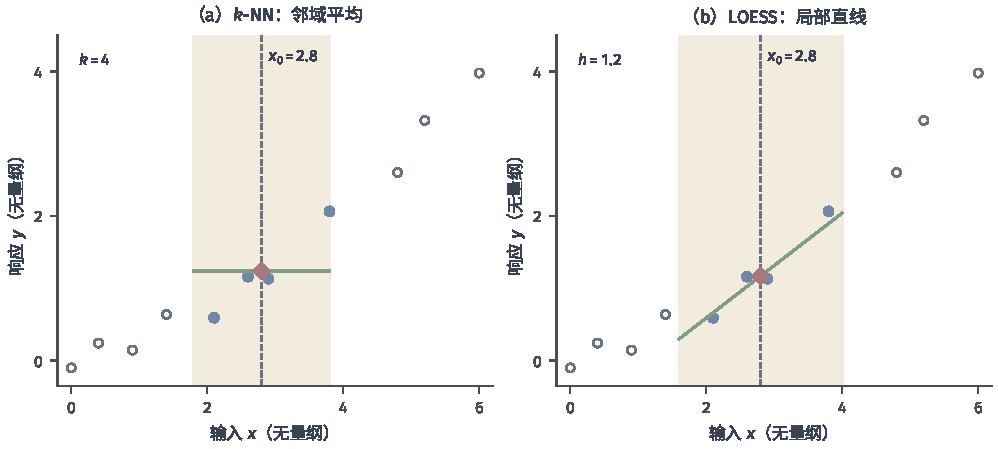
\includegraphics[width=159.059mm]{figures/04-classic-models/00-shared/matplotlib/regression-neighborhood/figure.pdf}
  \caption{同一查询点上的邻域平均与局部线性拟合。横、纵轴均无量纲，所有点均为构造样本；空心点为未使用样本，蓝色实心点为本次使用的四个样本，菱形为$x_0=2.8$处的预测。左图取$k=4$、等权平均，预测约为$1.238$；右图取$h=1.2$与三立方距离权重，不做残差重加权，局部线性预测约为$1.171$。浅色带标出各自的邻域，两图同时改变了局部函数形式和权重，不据此断言某种方法总是更准。}
  \label{fig:regression-neighborhood}
\end{figure*}

\subsubsection{参数学习}

设局部基设计为$\bm{P}$，权重矩阵为$\bm{W}=\operatorname{diag}(K_i)$。若$\bm{P}^{\top}\bm{W}\bm{P}$可逆，便可解加权正规方程得到局部系数；实际使用$\bm{W}^{1/2}\bm{P}$的QR分解等方法更合适。邻域无样本或有效点不足以确定多项式时，应扩大邻域、降低阶数或明确回退规则，不能直接使用逆矩阵公式。

一维局部线性形式可写得更清楚。令$u_i=x_i-x_0$，$S_j=\sum_iK_iu_i^j$、$T_j=\sum_iK_iu_i^jy_i$，并记$\Delta=S_0S_2-S_1^2$。方程组为
\[
  \begin{pmatrix}S_0&S_1\\S_1&S_2\end{pmatrix}
  \begin{pmatrix}\widehat a\\\widehat b\end{pmatrix}
  =\begin{pmatrix}T_0\\T_1\end{pmatrix}.
\]
若$\Delta>0$，查询点上的截距可表示为
\begin{equation}
  \widehat m(x_0)=\sum_i l_i y_i,\qquad
  l_i=\frac{K_i(S_2-u_iS_1)}{\Delta}.
  \label{eq:regression-local-linear-weights}
\end{equation}
对非负核权重，$\Delta=\sum_{i<j}K_iK_j(u_i-u_j)^2$，所以至少需要两个不同输入具有正权重。即使$\Delta>0$，接近退化的设计也可能产生很大的$l_i$。

固定带宽与只依赖输入的权重时，估计是响应$\bm{y}$的线性函数。若一个查询使用$n_{\mathrm{loc}}$个有效样本、$q$个局部基函数，稠密拟合约需$O(n_{\mathrm{loc}}q^2+q^3)$运算，另加邻域查询成本。

\subsubsection{局部斜率的作用与代价}
\label{sec:regression-loess-theory}

由式\eqref{eq:regression-local-linear-weights}求和可得$\sum_i l_i=1$、$\sum_i l_i(x_i-x_0)=0$。所以对于一次函数$m(x)=a+bx$，即使邻居都在查询的一侧，仍有$\sum_i l_i m(x_i)=m(x_0)$；局部斜率消去了平均输入不等于查询输入带来的一阶偏差。对光滑曲线，Taylor展开的常数项与一次项同样被再现，剩下的是曲率与更高阶变化。

这种补偿可能需要负权重。前面的两个单侧样本在$x_0=0$处给出$(l_1,l_2)=(2,-1)$，因此能从$0.1,0.2$外推到零。若两个响应分别含独立方差$\sigma^2$的噪声，局部线性预测方差为$(2^2+(-1)^2)\sigma^2=5\sigma^2$，等权平均则为$\sigma^2/2$。一般固定输入下，噪声方差为$\sum_i l_i^2\operatorname{Var}(Y_i\mid x_i)$；减少偏差可能增大方差，最终要由验证决定带宽与阶数\scite{fan1996local}。

\subsubsection{局部常数与稳健局部拟合}

\paragraph{用局部常数减少拟合参数}
\label{sec:regression-nadaraya-watson}

邻域中若只有一个有效输入，局部斜率无法确定；即使样本更多，估计斜率也可能带来不需要的噪声放大。只保留局部常数就能减少待估参数，同时保留按距离区别观测的方式。在式\eqref{eq:regression-local-polynomial}中只拟合截距，对截距求导便得到\term{Nadaraya--Watson核平滑}（Nadaraya--Watson kernel smoothing）
\begin{equation}
  \widehat m_{\mathrm{NW}}(\bm{x}_0)
  =\frac{\sum_iK_i y_i}{\sum_iK_i},
  \qquad \sum_iK_i>0.
  \label{eq:regression-nw}
\end{equation}
它与局部多项式使用相同的邻域权重，但只作加权平均。Nadaraya与Watson分别研究了这一核回归路线；具体带宽和设计条件仍须与所用理论结果对应\scite{nadaraya1964,watson1964}。

它保留非负权重与响应平均，计算比局部斜率简单；代价是不能自动抵消单侧邻域的线性趋势。局部常数、局部线性不是准确率的固定排序，而是不同局部信息与噪声下的取舍。

\paragraph{减弱异常响应对局部回归曲线的拉动}
\label{sec:regression-loess-robustness}

距离近不意味着响应可靠：查询附近的一条异常成交记录仍可能拉动整段拟合曲线。Cleveland的稳健LOESS先按距离作局部拟合，再根据残差增加降权系数，减小残差很大的记录在下一轮拟合中的作用。重复这两步后，局部曲线同时反映输入的远近和响应对当前曲线的偏离程度。

例如双权残差权重可取$a_i=[1-(r_i/c)^2]^2\mathbf1\{|r_i|<c\}$，其中$r_i=y_i-\widehat m(\bm x_i)$、$c>0$由残差尺度与验证设定。先在各训练输入处得到当前曲线与残差，算出$a_i$，再对每个查询将原距离权重改为$K_i a_i$，重新解局部加权问题。反复更新时检查局部秩和曲线变化，限制迭代次数；距离权重负责输入远近，残差权重负责当前拟合中的响应偏离，不能只算一次残差就声称已完成整个稳健过程。

残差权重依赖响应，整体估计便不再是固定的线性平滑算子，本节的固定权重方差公式不能直接沿用。这种处理针对异常响应；若局部输入覆盖不足，或异常输入支配了局部设计，残差降权本身不能补足信息。它也增加了重复拟合的计算成本，不能与只按输入设置带宽混为同一步骤。

\subsection{局部平均与局部拟合的关系}

$k$-NN用邻居数决定局部范围，距离加权和Nadaraya--Watson再区别邻居贡献；LOESS还在查询附近学习斜率或曲率。它们都保留训练记录参与预测，距离设定决定哪些记录提供依据，局部模型决定如何使用这些依据。搜索索引减少找邻居的工作，却不能代替LOESS每次查询的局部求解；稳健残差权重也不能补足没有数据的区域。

\section{基于树与规则的回归}
\label{sec:regression-trees}

第\ref{sec:classic-overview-tree-rules}节已经给出条件分支与区域预测的共同结构。本节关注回归时怎样按响应损失选择区域，并确定叶内预测。CART采用递归划分，模型树在叶内加入线性趋势，MARS用连续铰链基表达阈值及交互。MARS的基函数可以重叠，并不构成标准决策树；把它放在这里，是为了比较不同的条件与分段表达。

\subsection{CART 回归树}
\label{sec:regression-cart}

有些响应变化来自明确的条件组合，未必适合用全局直线或平滑邻域描述。考虑一个教学函数：只有$x_1>1/2$且$x_2>1/2$时响应为$10$，其他区域为$0$。固定$x_2\leq1/2$时，改变$x_1$不起作用；固定$x_2>1/2$时，越过$x_1=1/2$却使响应跳变。一个全局斜率无法同时表达这两种作用，平滑曲线也会在跳变附近折中。先按$x_2$分支，再在高值分支按$x_1$分支，就能用三个常数区域精确表示这个函数。

\term{分类与回归树}（classification and regression trees, CART）让数据选择这样的阈值与分支，并将递归二分、叶内估计和复杂度剪枝组织成统一框架。Breiman等人在1984年的专著中系统阐述了这套方法，把数据决定的分区与树的规模控制联系起来。回归情形通常用平方误差评价分裂，再通过独立验证选择树的规模；这一流程将在下面分别展开\scite{breiman1984cart}。

第\ref{sec:classification-cart}节的分类CART共享递归二分与代价复杂度剪枝。任务差异落在分裂和叶输出上：本节按响应平方误差选择分区并输出叶均值，分类树按类别不纯度或误分类代价分裂，并输出类别标签或类别比例。

\subsubsection{模型结构}

设树$T$的叶区域为$R_1,\ldots,R_M$，则
\begin{equation}
  f_T(\bm{x})=\sum_{m=1}^{M}c_m\mathbf{1}\{\bm{x}\in R_m\}.
  \label{eq:regression-cart-model}
\end{equation}
数值特征上的节点规则通常为$x_j\leq s$与$x_j>s$，递归后形成轴对齐区域；类别特征则可按类别子集分支，不宜继续称为普通欧氏矩形。缺失值并非由树结构自动解决，还需指定缺失方向或其他规则。例如，\term{替代分裂}（surrogate split）在主测试特征缺失时，用其他特征的测试尽量复现主分裂的左右分配。

固定非空叶的样本索引集$I_m$后，令$\bar y_m=|I_m|^{-1}\sum_{i\in I_m}y_i$，有
\[
  \sum_{i\in I_m}(y_i-c)^2
  =\sum_{i\in I_m}(y_i-\bar y_m)^2+|I_m|(c-\bar y_m)^2.
\]
因此$c_m=\bar y_m$在平方损失下最优。改用绝对或分位数损失时，叶预测相应变为中位数或分位数；模型结构与损失选择仍然可以分开。

图\ref{fig:regression-tree-prediction}把一棵给定的阈值树展开为预测函数。沿树走到同一叶的输入共享一个预测值，所以一维常数叶回归树产生水平分段，而阈值处可以跳跃。图中每个叶的数值都来自该叶的两条响应，后面的学习问题才是如何从候选阈值中选出这些分区。

\begin{figure*}[t]
  \centering
  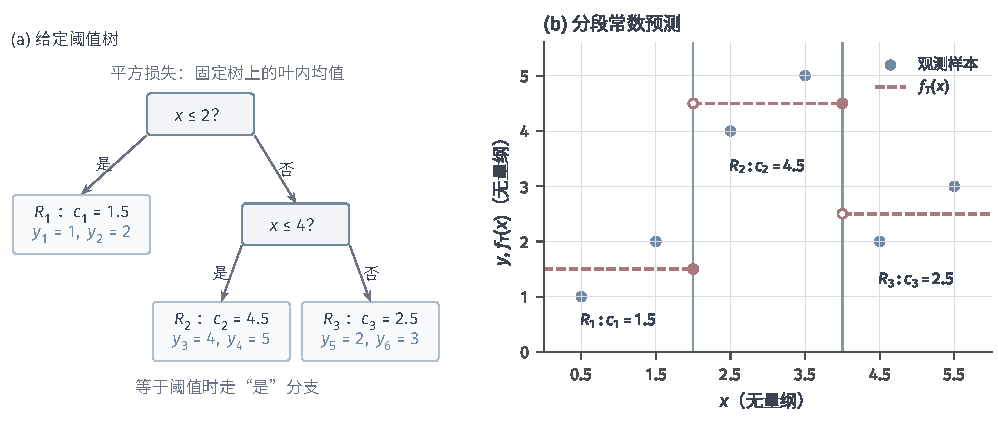
\includegraphics[width=159.059mm]{figures/04-classic-models/00-shared/matplotlib/regression-tree-prediction/figure.pdf}
  \caption{给定阈值树与分段常数预测。六个无量纲教学样本按$x$递增排列；按$x\leq2$及右分支上的$x\leq4$划分后，三组响应分别为$(1,2)$、$(4,5)$、$(2,3)$，叶均值为$1.5$、$4.5$、$2.5$。蓝色点表示样本，红色虚线表示预测，绿色竖线表示阈值；阈值处实心、空心端点区分取与不取该值。右图只显示$0\leq x\leq6$，树结构预先给定。}
  \label{fig:regression-tree-prediction}
\end{figure*}

\subsubsection{参数学习}
\label{sec:regression-cart-learning}

在当前节点内，算法枚举特征与候选阈值，选择子节点平方误差和最小的分裂。直观上，只要一个分裂能把响应均值明显不同的两群样本分开，让每群各自用自己的均值作预测，就比全体共用一个均值更贴合；若两群均值相同，分开就没有收益。对两个非空子节点，记样本数为$n_L,n_R$，均值为$\bar y_L,\bar y_R$，则分裂增益（父节点平方误差减去两个子节点平方误差之和）可精确写成
\begin{equation}
  \Delta_{\mathrm{split}}
  =\mathrm{SSE}_{\mathrm{parent}}
    -\mathrm{SSE}_{L}-\mathrm{SSE}_{R}
  =\frac{n_Ln_R}{n_L+n_R}(\bar y_L-\bar y_R)^2.
  \label{eq:regression-cart-gain}
\end{equation}
证明只需把两个子节点响应分别围绕自己的均值展开，再利用父均值为加权平均。该式说明增益同时考虑两组均值差异和样本量。

连续特征只需在相邻不同取值之间设候选切分，排好序后用累计和、平方和更新各侧SSE。类别子集有更多候选；在无额外分裂约束的平方误差二分问题中，可先按类别响应均值排序再考虑相邻分组，但带最小样本数、权重或其他限制时须重新检查相应结论。停止条件可限制最大深度、最小叶样本数和最低增益。贪心选择只保证当前节点在候选集中的最佳切分，不保证整棵树全局最优。

树一直生长下去，每片叶最终只剩一两个样本，训练误差可以降到零，但这只是把每条训练记录单独背下来，对新样本毫无意义。控制规模有两种时机：生长中途提前停止，或先让树充分长大、再回过头剪掉多余的分支。后者通常更稳妥——某些分裂单看一步收益很小，却能为下一步很有价值的分裂创造条件，提前停止会把这类结构一并错过；先长后剪则是在看到整棵树之后作全局取舍。固定一个已生长的有限二叉树$T_0$，用参数$\alpha$表示“每多保留一片叶需要付出的代价”，对其剪枝子树$T$定义
\begin{equation}
  R_\alpha(T)=\sum_{m\in\operatorname{leaves}(T)}
                    \mathrm{SSE}_m+\alpha|\operatorname{leaves}(T)|,
  \qquad\alpha\geq0.
  \label{eq:regression-pruning}
\end{equation}
$\alpha=0$时代价项为零，保留全部叶的大树最划算；$\alpha$增大，叶数多的树被罚得更重，更小的树逐渐成为最优，于是调节$\alpha$就能得到一列从复杂到简单的候选子树，再由验证集选出合适的规模。
\term{代价复杂度剪枝}（cost-complexity pruning）在保留局部拟合与减少叶数之间作折中。临界$\alpha$处可能出现多个最优子树，唯一性需要额外的并列规则。

\Needspace{11\baselineskip}
\begin{theorem}[CART在固定生长树内的最优剪枝解]
  \label{thm:regression-pruning}
  设$Q_\alpha(v)$为从$T_0$的节点$v$出发可得到的所有剪枝子树的最小代价。若$v$是原始叶，则$Q_\alpha(v)=\mathrm{SSE}_v+\alpha$；若$v$有左右孩子$v_L,v_R$，则
  \[
    Q_\alpha(v)=\min\{\mathrm{SSE}_v+\alpha,\,
                     Q_\alpha(v_L)+Q_\alpha(v_R)\}.
  \]
  从叶到根计算该递推，并保存每次选择，可得到$R_\alpha$的最优剪枝子树。
\end{theorem}

\begin{proof}
原始叶无其他选择，结论成立。对内部节点，任何合法剪枝子树要么把$v$收缩为一片叶，要么保留分裂。前者代价为$\mathrm{SSE}_v+\alpha$；后者的两个孩子可以独立剪枝，代价相加，归纳假设给出最小和为$Q_\alpha(v_L)+Q_\alpha(v_R)$。这两类穷尽全部选择，因此取最小值即可。相等时两个选择都最优，记录任一个并列规则均可返回一个最优解。
\end{proof}

固定$\alpha$时，递推只需对每个节点作常数次比较，因此在节点SSE已知后为$O(|T_0|)$。经典最弱环节方法进一步构造随$\alpha$变化的嵌套剪枝路径，再通过验证选择规模；它优化的仍是给定生长树内的剪枝集合，而不是所有可能的树。交叉验证时，各折的生长与剪枝都应仅使用该折训练集。

\subsubsection{分区选择与叶内趋势}
\label{sec:regression-cart-theory}

有限片常数适合表示阈值变化，却不擅长用少量叶描述连续斜率。例如$m(x)=1+2x$可由一个线性模型精确表示，常数叶必须继续切分才能逐渐逼近。另一方面，叶越来越小，估计其均值的记录也越来越少。树的深度、叶样本数和剪枝参数因此需要通过完整的训练—验证流程选择。

分裂使用了响应，不能在选完树后就把各叶当成事先固定的独立样本组，直接宣称叶均值无偏或方差只等于$\sigma^2/n_m$。独立数据分别选分区与估计叶均值，可以分离这两项选择，但普通CART并不自动具有这种安排。贪心分裂还可能错过需要联合考察的交互；后续Bagging、随机森林和提升树改变成员生成与组合，以处理不同的误差来源。

\label{sec:regression-model-tree}

如果区域内部仍有连续的线性变化，常数叶就需要继续切分。我们可以保留树对不同条件的分区，让每片叶负责拟合该区域内部的趋势。\term{模型树}（model tree）在叶内拟合线性模型$f_m(\bm{x})=b_m+\bm{w}_m^{\top}\bm{x}_{A_m}$，其中$A_m$为该叶使用的特征集。M5是这条路线的代表，用树选择适用区域，再用局部回归描述区域内部的趋势\scite{quinlan1992m5}。

固定分区后，第$m$片叶只用本叶记录最小化$\sum_{i:\bm x_i\in R_m}(y_i-b_m-\bm w_m^\top\bm x_{i,A_m})^2$，用OLS或带正则的线性求解得到系数；新输入先沿树找到叶，再计算该叶的线性预测。若分裂阶段就要按线性叶评价候选，可以对每个候选子区域分别重拟合叶模型，比较两侧总残差；此时不能继续把常数叶均值的式\eqref{eq:regression-cart-gain}当成该增益。分区、叶内特征与正则强度要和剪枝一起由训练内验证决定，不同模型树实现可采用不同搜索与平滑规则。

局部样本少时，叶内设计可能秩亏，需要选择变量或正则化。父子节点预测的加权混合可以缓和估计跳跃，但两侧叶模型在共同边界上没有被强制相等，因此这种平滑处理不自动保证函数连续。叶模型也可改为GLM、岭或Lasso，不过分裂准则、参数估计与复杂度惩罚需要与新模型配套，不能只替换叶公式就沿用全部CART理论。



\subsection{多元自适应回归样条（MARS）}
\label{sec:regression-mars}

树的阈值选择能够适应数据，常数叶却在边界处跳跃：跨过阈值的输入哪怕只差一点点，预测也会突然跳到另一个水平。很多真实关系并没有这种突变——比如价格随面积变化时，更常见的是斜率在某处发生改变，而不是价格整体跳一档。如果希望保留“阈值由数据自动确定”的好处，又让预测在跨过阈值时保持连续，可以让阈值处只改变之后直线的斜率，而不改变函数值本身。例如$m(x)=1+2x+3(x-1)_+$在$x\leq1$时斜率为$2$，在$x>1$时斜率为$5$；$(x-1)_+$在结点处从零开始增长，所以没有产生跳跃。常数叶需要许多区域来逼近这段线性变化，两个斜率和一个结点却已能准确描述它。\term{多元自适应回归样条}（multivariate adaptive regression splines, MARS）把阈值写进连续的铰链基函数，再从数据中选择这些基函数及其乘积。Friedman在1991年提出这一方法，将自适应选择结点与样条展开结合。它在可加模型与树式区域表达之间提供了另一种选择：多个基函数可同时作用于同一输入，预测不再由唯一一片叶决定\scite{friedman1991mars}。

\subsubsection{模型结构}

对特征$x_j$与结点$t$，\term{铰链函数}（hinge function）为$(x_j-t)_+$与$(t-x_j)_+$，它们在结点一侧为零，另一侧线性变化。MARS写成
\begin{equation}
  f(\bm{x})=\beta_0+\sum_{m=1}^{M}\beta_m B_m(\bm{x}),
  \qquad
  B_m(\bm{x})=\prod_{l=1}^{q_m}
                 [s_{m,l}(x_{j_{m,l}}-t_{m,l})]_+,
  \label{eq:regression-mars}
\end{equation}
其中$s_{m,l}\in\{-1,1\}$，$q_m$为该基的因子数。通常限制最高交互阶数，并对同一乘积中重复使用变量设规则，避免无约束扩张。下面采用每个乘积只使用互异变量的基本版本，因此$q_m$同时表示该基涉及的变量数；它不能超过预先给定的最高交互阶数$1\leq q_{\max}\leq d$。其他允许重复变量或平滑基的实现，需要另行说明自己的候选规则。

单个铰链连续但在结点不可微；含两个不同变量的乘积如$(x_1-3)_+(5-x_2)_+$在激活区域是二次乘积，不再是整体分段线性函数。铰链和乘积都连续，所以有限线性组合连续，但可微性需要额外平滑构造。严格加性版本只允许单变量基，增加乘积则允许指定阶数内的交互。

\subsubsection{参数学习}

前向阶段从常数模型开始，把已有基$B_l$与一对左右铰链相乘，尝试加入$B_l(\bm x)(x_j-t)_+$和$B_l(\bm x)(t-x_j)_+$。父基与其他已有基仍保留，区别于树用两个孩子替换一个叶。候选变量不能已出现在该乘积中，新增因子数不能超过$q_{\max}$；候选结点取父基非零区域内的不同训练取值，并要求结点两侧都有预定数量的观测支持。

对每个合法候选，都把新旧基一起组成设计矩阵，重新用QR或SVD拟合线性系数，再比较训练SSE。选取下降最多的一对后继续扩展，直到基数量达到上限、没有合法候选或改善不足。并列候选采用固定规则。比如父基为$(x_1-t_1)_+$时，在新变量$x_2$上扩展会增加只在$x_1>t_1$区域起作用的交互斜率；这个局部条件来自基的乘积，而不是唯一一条树路径。

后向阶段逐次尝试删除非截距基，每步保留训练误差增加最少的删除，形成由大到小的一串模型，并在每步重新拟合剩余系数。最后用验证误差或广义交叉验证选择规模。常用准则为

\begin{equation}
  \operatorname{GCV}
  =\frac{\mathrm{SSE}/n}{(1-C_{\mathrm{eff}}/n)^2},
  \qquad C_{\mathrm{eff}}<n.
  \label{eq:regression-mars-gcv}
\end{equation}
$C_{\mathrm{eff}}$是复杂度计数，既考虑保留的线性系数，也以附加惩罚近似结点搜索的代价。例如可写成$q+cK$，其中$q$是保留设计的秩，$K$是采用相应计数约定的结点数，$c$是每个结点的附加代价。软件对成对基、交互结点与自由度有不同计数方式，使用GCV前需要明确采用哪种复杂度计数；该计数近似了搜索代价，区别于自适应拟合的精确自由度。

\subsubsection{连续性、交互与搜索的边界}

增加结点能够改变单变量曲线的分辨率，增加乘积的变量数才能引入新的交互；两者不能互相替代。只允许单变量项时，MARS与GAM一样不能表达一般的$x_1x_2$作用；允许二阶乘积后，可以利用$x=(x)_+-(-x)_+$把这个交互展开为四个铰链乘积。固定基的系数拟合是最小二乘，选择哪些基却是离散的贪心搜索，局部改善不等于搜索全部结构后的全局最优。

结点和基由响应参与选择，GCV中的复杂度计数只是对搜索代价的近似，不能把被选中的基当作抽样前固定。应限制基数量和交互阶数，并用未参与搜索的验证记录比较。基本MARS连续但未必可微；铰链在观测范围外继续线性增长，外推需要另作检查。

\subsection{树、线性叶与铰链展开}

输入跨过阈值以后，预测可能切换到新的水平，也可能只改变斜率。CART用常数叶表达前一种情况；若区域内还有连续趋势，模型树在同一叶中增加线性项，减少为了描述斜率而继续切分的需要。MARS则把阈值写成连续铰链，允许多个基函数及其乘积共同作用于一个输入。模型树的不同叶仍可能在边界跳跃，MARS的基本构造连续但不必处处可微；前者按路径查询并估计各叶系数，后者计算保留的全部基。需要的局部样本、交互搜索和预测成本因而不同。

树的变量选择还可能偏向具有较多候选切分的特征。\term{条件推断树}（conditional inference tree）把变量关联检验与分裂位置选择分开，缓解候选切分多的变量更容易被选中的偏向；检验规则和显著性水平共同控制树大小，预测误差仍需由样本外评价确定\scite{hothorn2006ctree}。

\section{基于概率的回归}
\label{sec:regression-probabilistic}

一个房价点预测没有说明价格自身的波动，也没有说明有限数据下函数估计的差异。GLM已经通过条件分布描述前一种变化；本节进一步给未知系数或函数设置先验，由观测形成后验，再将函数不确定性与响应噪声一起带入预测分布。第\ref{sec:classic-overview-probabilistic}节的概率表示由此落实为可以计算的后验更新。

为什么需要把“函数”本身当作随机对象，而不只是估计一组固定系数？因为点预测给出的单个数值无法表达“这个预测有多可靠”：同一区域两套房屋可能给出相同的预测价格，但其中一处紧邻大量成交记录、估计很有把握，另一处远离任何观测、基本是在猜测，只看一个数字无法分辨二者。有限维基模型可以给系数设置分布来描述这种不确定性，但曲线形状从此被预先选定的基限死。如果希望直接用“相近输入处的函数值应当怎样一起起伏”来规定未知曲线的所有可能形状，就可以把概率模型建立在函数值上。

\subsection{高斯过程回归（GPR）}
\label{sec:regression-gpr}

点预测给出一个数值，却没有说明训练数据在该位置提供了多少信息。两个输入都得到相同价格预测，其中一个可能紧邻大量观测，另一个却远离训练范围；仅看这两个数值，无法分辨估计的不确定性。给有限基系数设置分布，可以描述未知系数带来的变化，但函数形状仍受预先选定的基限制。如果希望直接用“相近输入处的函数值怎样一起变化”来规定未知曲线，就可以把概率模型建立在函数值上。\term{高斯过程回归}（Gaussian process regression, GPR）用均值函数规定各位置的先验中心，用协方差函数规定函数值怎样共同变化。任意有限输入集合上的函数值都具有联合高斯分布，加入高斯观测噪声以后，可以精确计算后验与预测分布。先从有限权重模型推导这一计算，再转向函数值本身，就能看清它与贝叶斯线性回归、核岭回归的联系。

高斯过程预测较早已用于时间序列和地统计学，空间预测中的相关方法通常称为克里金（kriging）。20世纪90年代，Williams与Rasmussen在机器学习语境中讨论了GPR及协方差函数参数的学习，并将它与贝叶斯神经网络联系起来\scite{rasmussen2006}。

\subsubsection{模型结构}
\label{sec:regression-gpr-structure}

先考虑有限维特征$\bm\phi(\bm x)\in\mathbb R^p$，令$f(\bm x)=\bm\phi(\bm x)^\top\bm w$。OLS给出一组拟合系数，岭回归还会用惩罚规定哪些系数较可接受；如果要让预测保留这些未知系数的全部分布，而不是只保留一个点，就可以先设置系数的先验分布，再用观测更新。\term{贝叶斯线性回归}（Bayesian linear regression）采用这种做法。

考虑只含截距的教学模型。我们先给未知均值设置均值为$100$、方差为$20^2$的高斯先验，再将单次观测噪声的方差设为$10^2$。观测到一次$100$以后，后验均值仍是$100$，但后验方差从$400$降为$(1/400+1/100)^{-1}=80$。点预测没有变化，观测却减少了不确定性；预测下一次带噪响应时还要加上$100$的观测噪声方差。下面将这一计算推广到多个系数，使用高斯先验与高斯噪声通过完成平方求出后验。

这个方差更新可以直接从两个密度看出。若把未知截距记为$b$，先验密度与这一次观测的似然相乘，得到与$\exp\{-\tfrac12(b-100)^2(1/400+1/100)\}$成正比的后验密度。括号中的系数是方差的倒数，称为精度；它越大，密度越集中。这里先验和数据提供的精度相加，所以新的方差是精度之和的倒数。若观测值与先验中心不同，完成平方还会把中心改成按两种精度加权的平均。下面的矩阵公式保留相同机制：协方差的逆矩阵描述各参数方向的精度，观测通过设计矩阵提供额外信息。

\Needspace{14\baselineskip}
\begin{lemma}[贝叶斯线性回归的后验与预测]
  \label{thm:regression-bayesian-linear}
  条件于设计矩阵$\bm{X}$，设$\bm{w}\sim\mathcal{N}(\bm{m}_0,\bm{V}_0)$，其中$\bm{V}_0\succ0$，并设$\bm{y}=\bm{X}\bm{w}+\bm{\varepsilon}$，$\bm{\varepsilon}\sim\mathcal{N}(\bm{0},\sigma^2\bm{I})$与$\bm{w}$独立，$\sigma^2>0$。则
  \[
    \begin{aligned}
      \bm{V}_n&=(\bm{V}_0^{-1}+\sigma^{-2}\bm{X}^{\top}\bm{X})^{-1},\\
      \bm{m}_n&=\bm{V}_n
          (\bm{V}_0^{-1}\bm{m}_0+\sigma^{-2}\bm{X}^{\top}\bm{y}),
    \end{aligned}
  \]
  且$\bm{w}\mid\bm{X},\bm{y}\sim\mathcal{N}(\bm{m}_n,\bm{V}_n)$。新响应采用独立同方差噪声时，
  \[
    Y_{\star}\mid\bm{x}_{\star},\bm{X},\bm{y}
    \sim\mathcal{N}\bigl(
      \bm{\phi}_{\star}^{\top}\bm{m}_n,\,
      \bm{\phi}_{\star}^{\top}\bm{V}_n\bm{\phi}_{\star}+\sigma^2\bigr).
  \]
\end{lemma}

\begin{proof}
给定设计以后，后验密度正比于先验密度与似然的乘积。先保留两个二次项的原形，其负对数除去常数为
\[
 \tfrac12(\bm w-\bm m_0)^\top\bm V_0^{-1}(\bm w-\bm m_0)
 +\frac1{2\sigma^2}(\bm y-\bm X\bm w)^\top(\bm y-\bm X\bm w).
\]
第一项衡量参数偏离先验中心的程度，第二项衡量这些参数与观测的符合程度。分别展开这两个平方，把所有含$\bm w$的二次项和一次项合并，就得到下面的配方起点。
先验与似然的负对数相加，去掉与$\bm{w}$无关的项后为
\[
  \tfrac12\bm{w}^{\top}
       (\bm{V}_0^{-1}+\sigma^{-2}\bm{X}^{\top}\bm{X})\bm{w}
  -\bm{w}^{\top}
       (\bm{V}_0^{-1}\bm{m}_0+\sigma^{-2}\bm{X}^{\top}\bm{y}).
\]
定义引理中的$\bm{V}_n,\bm{m}_n$，上式等于
$\tfrac12(\bm{w}-\bm{m}_n)^{\top}\bm{V}_n^{-1}(\bm{w}-\bm{m}_n)$加常数。这是因为展开该平方后的一次项为$-\bm w^\top\bm V_n^{-1}\bm m_n$，而引理恰好令$\bm V_n^{-1}\bm m_n=\bm V_0^{-1}\bm m_0+\sigma^{-2}\bm X^\top\bm y$。先验精度正定，似然贡献的$\sigma^{-2}\bm X^\top\bm X$半正定，两者相加仍正定，故该可积密度归一化后就是所述高斯后验。新响应为后验高斯参数的线性变换与独立高斯噪声之和；线性变换的均值为$\bm\phi_\star^\top\bm m_n$、方差为$\bm\phi_\star^\top\bm V_n\bm\phi_\star$，再加上新噪声的方差即得预测分布。
\end{proof}

若只需用一个参数向量概括后验，可取当前参数化下的后验众数，即最大后验估计（MAP）。固定设计与超参数，且最大值能够取到时，当前回归模型的目标为
\begin{equation}
  \begin{aligned}
    \widehat{\bm{w}}_{\mathrm{MAP}}
      &\in\argmax_{\bm{w}}p(\bm{w}\mid\bm{X},\bm{y})\\
      &=\argmax_{\bm{w}}
        \{\log p(\bm{y}\mid\bm{X},\bm{w})+\log p(\bm{w})\}.
  \end{aligned}
  \label{eq:regression-map}
\end{equation}
后验的归一化常数与$\bm{w}$无关，因而不影响最大化。MAP使用后验众数，后验均值则对参数按后验加权平均，两者一般不同。

图~\ref{fig:regression-mle-map-geometry}在二维参数平面上展示这两个目标的差别。似然单独把最优点放在数据偏好的中心；零均值先验则偏好靠近原点的参数。MAP最小化负对数似然与负对数先验之和，因此落在二者共同决定的位置，而不是在MLE与先验中心之间任意作线性插值。椭圆形状和先验尺度改变时，折中的方向也会改变。
\begin{figure}[htbp]
  \centering
  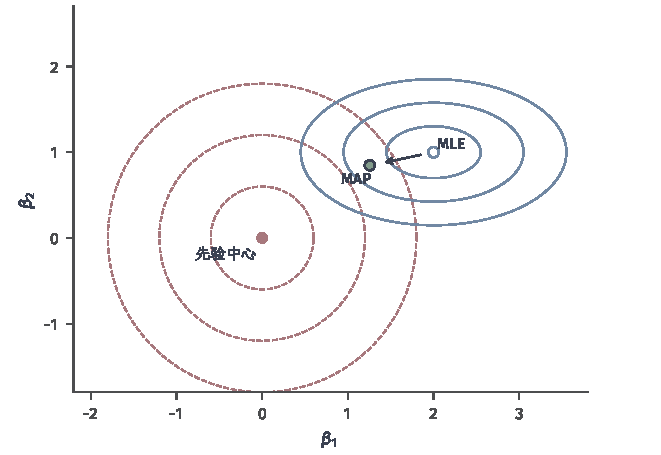
\includegraphics[width=105.412mm]{figures/04-classic-models/00-shared/matplotlib/regression-mle-map-geometry/figure.pdf}
  \caption{MLE与MAP的参数几何。蓝色实线是以$(2,1)^\top$为中心、两坐标尺度分别为$1$和$0.55$的高斯似然等高线；红色虚线是以原点为中心、尺度为$1.3$的各向同性高斯先验等高线。空心点为MLE，绿色实心点为两项相加后的MAP，坐标保留三位小数为$(1.257,0.848)^\top$。该构造用于显示先验如何改变点估计，不代表MAP总在两中心的连线上。}
  \label{fig:regression-mle-map-geometry}
\end{figure}

若$\bm{m}_0=\bm{0}$、$\bm{V}_0=\tau^2\bm{I}$，后验均值为$(\bm{X}^{\top}\bm{X}+\sigma^2\bm{I}/\tau^2)^{-1}\bm{X}^{\top}\bm{y}$，在本章归一化下对应$\lambda=\sigma^2/(n\tau^2)$的岭估计。高斯后验的均值与众数相同，所以也等于MAP估计。该对应要求截距处理一致：若先验惩罚全部特征系数，就不能直接与截距不受惩罚的岭模型比较。

后验协方差描述在当前先验与噪声模型中，观察数据后参数仍有多大不确定性；它不同于固定真参数、反复生成训练噪声时岭系数的协方差。高斯后验预测区间也依赖模型设定，不能直接当作任意真实函数下的覆盖保证。

有限维贝叶斯线性模型已经诱导出函数上的高斯分布：
\[
  m_0(\bm{x})=\bm{\phi}(\bm{x})^{\top}\bm{m}_0,\qquad
  k(\bm{x},\bm{x}')=\bm{\phi}(\bm{x})^{\top}\bm{V}_0\bm{\phi}(\bm{x}').
\]
任意有限个函数值都是高斯参数的线性变换，因此联合高斯。直接指定$m_0$和正定核$k$，便可越过显式系数建立函数先验。

把这一关系推广为$f\sim\mathcal{GP}(m_0,k)$：不再预先选定有限个基函数，而是直接对“任意位置上的函数值”规定一条概率律——在任意选取的有限个输入位置上，对应的函数值向量都服从联合高斯分布，其均值由$m_0$给定、任意两个位置之间的协方差由$k$给定。可以这样理解它：一条未知曲线在无穷多个位置上都有取值，我们无法把这无穷多个数都当成待估参数，但只需要保证“随便挑出有限个位置，它们的取值都服从一个由$m_0$和$k$决定的多元高斯”，整条曲线的随机规律就被完整规定了。同一个$m_0$和$k$保证删去或重排输入时，所得边缘分布彼此一致。核可以有限秩，因此贝叶斯线性回归正是一个特例；无限维核也只需通过有限函数值的联合分布计算，不必先列出无限多个权重。

加入与函数独立的噪声$y_i=f(\bm{x}_i)+\varepsilon_i$，其中$\varepsilon_i$相互独立且服从$\mathcal{N}(0,\sigma^2)$，$\sigma^2>0$。令$\bm{K}_{i,j}=k(\bm{x}_i,\bm{x}_j)$，$(\bm{k}_{\star})_i=k(\bm{x}_i,\bm{x}_{\star})$，$\bm{m}_0$表示训练点上的先验均值向量，$\bm{C}=\bm{K}+\sigma^2\bm{I}$，$f_{\star}=f(\bm{x}_{\star})$。联合分布为
\[
  \begin{pmatrix}\bm{y}\\f_{\star}\end{pmatrix}
  \sim\mathcal{N}\!\left[
    \begin{pmatrix}\bm{m}_0\\m_0(\bm{x}_{\star})\end{pmatrix},
    \begin{pmatrix}
      \bm{C}&\bm{k}_{\star}\\
      \bm{k}_{\star}^{\top}&k(\bm{x}_{\star},\bm{x}_{\star})
    \end{pmatrix}\right].
\]
于是后验预测可以精确写成
\begin{equation}
  \begin{aligned}
    \mu_{\star}
      &=m_0(\bm{x}_{\star})
        +\bm{k}_{\star}^{\top}\bm{C}^{-1}(\bm{y}-\bm{m}_0),\\
    v_{\star}
      &=k(\bm{x}_{\star},\bm{x}_{\star})
        -\bm{k}_{\star}^{\top}\bm{C}^{-1}\bm{k}_{\star}.
  \end{aligned}
  \label{eq:regression-gp-posterior}
\end{equation}
为证明它，令$Z=f_{\star}-m_0(\bm{x}_{\star})-\bm{k}_{\star}^{\top}\bm{C}^{-1}(\bm{y}-\bm{m}_0)$。直接计算得到$\operatorname{Cov}(Z,\bm{y})=\bm{0}$；$Z$与$\bm{y}$联合高斯，所以独立。其方差为$v_{\star}$，从而条件于$\bm{y}$时，$f_{\star}$的均值为$\mu_{\star}$、方差为$v_{\star}$。该方差非负也由它是随机变量方差得到。未来带噪声响应的方差则为$v_{\star}+\sigma^2$。



核选择规定了先验中的相似性。平方指数核$k(\bm{x},\bm{x}')=\sigma_f^2\exp(-\lVert\bm{x}-\bm{x}'\rVert_2^2/(2\ell^2))$具有很强的平滑性，其中$\sigma_f^2>0$是信号方差、$\ell>0$是长度尺度。Matérn核可调节平滑程度，例如$\nu=3/2$时为$\sigma_f^2(1+\sqrt3r/\ell)\exp(-\sqrt3r/\ell)$，其中$r=\lVert\bm{x}-\bm{x}'\rVert_2$，对应一次均方可微的过程。一维周期核可写成$\sigma_f^2\exp(-2\sin^2(\pi(x-x')/p)/\ell^2)$，表达周期$p>0$的相关结构。合法核的和与乘积仍合法，可以组合趋势与周期，但不保证所组合的结构符合实际数据。

这些参数规定函数值怎样共同变化：$\sigma_f^2$控制偏离先验均值的幅度，$\ell$越大，相同距离上的函数值相关性越强；平方指数核的两个位置相距$\ell$时，相关系数为$\exp(-1/2)$。它与第\ref{sec:classic-overview-common-kernels}节高斯核参数的对应为$\beta=1/(2\ell^2)$。Matérn核允许调整平滑程度，周期核则编码相隔$p$后反复出现的关系。核相加可以对应独立GP分量相加；核相乘仍合法，但不能据此把两个GP样本函数的乘积也称为GP。

图\ref{fig:regression-gp-posterior}展示了式\eqref{eq:regression-gp-posterior}的两项输出。在这个固定平稳核的例子中，观测附近的函数值受到较强约束，观测间的较大空隙与远离观测的区域保留更多不确定性。曲线给出点预测，带状区域则说明在当前先验和噪声设定下，哪些函数值仍与数据相容。

\begin{figure}[htbp]
  \centering
  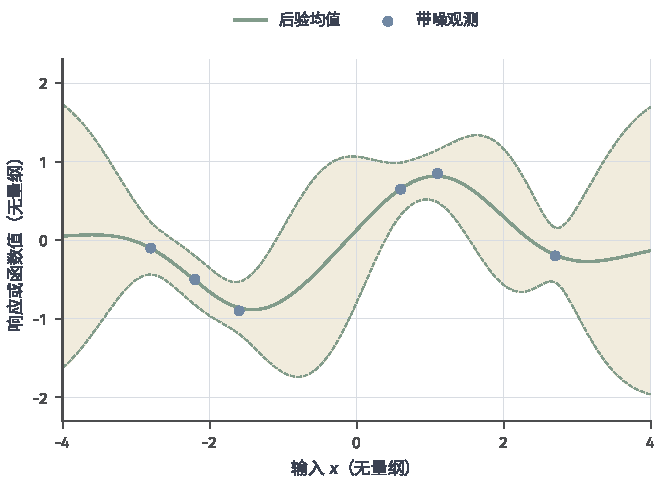
\includegraphics[width=105.412mm]{figures/04-classic-models/00-shared/matplotlib/regression-gp-posterior/figure.pdf}
  \caption{高斯过程的后验均值与函数不确定性。六个点为构造观测；先验均值为零，平方指数核取$\ell=0.9$、$\sigma_f=1$，观测噪声标准差为$\sigma=0.18$。实线为$\mu_{\star}$，浅色带及虚线边界为$\mu_{\star}\pm1.96\sqrt{v_{\star}}$，表示潜在函数值的逐点约$95\%$后验可信区间。它不是整条函数的同时可信带；预测未来带噪响应时，方差还须加$\sigma^2$。}
  \label{fig:regression-gp-posterior}
\end{figure}

\subsubsection{参数学习}
\label{sec:regression-gpr-learning}

给定核和噪声参数时，后验已经由式\eqref{eq:regression-gp-posterior}确定；仍需选择长度尺度、信号方差、噪声方差及可能的均值参数。为什么调这些超参数不能直接用训练拟合好坏，而要引入“边缘似然”？因为一条足够灵活的GP几乎可以穿过所有训练点，单纯追求拟合会把噪声方差调到零、长度尺度调到极小，得到一条剧烈振荡的曲线。合理的准则应当同时奖励“贴合观测”和“曲线本身平滑、不需要极端巧合”，边缘似然正好把这两点综合起来。令这些超参数为$\bm{\theta}$，把训练输入处的潜在函数值积分掉，得到\term{边缘似然}（marginal likelihood），即在给定输入和超参数时观测响应向量的概率密度——“积分掉”是指对先验允许的每一条可能的曲线，按它的先验概率加权，累加它产生当前观测的可能性，于是过于曲折、先验概率很低的曲线即使恰好穿过数据也不会占主导。以下令先验均值为零。
先把训练点上的潜在函数值记成$\bm f=(f(\bm x_1),\ldots,f(\bm x_n))^\top$，则这一积分写成
\[
 p(\bm y\mid\bm X,\bm\theta)
  =\int p(\bm y\mid\bm f,\bm X,\bm\theta)
         p(\bm f\mid\bm X,\bm\theta)\,d\bm f.
\]
积分中先按先验给每一组可能的函数值分配权重，再累加这些函数值产生当前观测的密度。零均值先验给出$\bm f\sim\mathcal N(\bm0,\bm K_{\bm\theta})$，独立高斯噪声与之相加，所以$\bm y\sim\mathcal N(\bm0,\bm C_{\bm\theta})$，其中$\bm C_{\bm\theta}=\bm K_{\bm\theta}+\sigma^2\bm I$。对这个$n$维高斯密度取对数，得到
\begin{equation}
  \log p(\bm{y}\mid\bm{X},\bm{\theta})
   =-\tfrac12\bm{y}^{\top}\bm{C}_{\bm{\theta}}^{-1}\bm{y}
    -\tfrac12\log|\bm{C}_{\bm{\theta}}|
    -\tfrac n2\log(2\pi).
  \label{eq:regression-gp-evidence}
\end{equation}
二次项评价响应与协方差结构的匹配，行列式项来自密度归一化，两者共同决定目标。行列式随核的尺度和相关结构变化，外层优化据此选择当前核族中的超参数；所选结构的预测效果仍需用样本外数据检查。

一维情形能说明为什么必须同时看这两项。若$Y\sim\mathcal N(0,c)$且$c>0$，去掉常数后的负对数密度为$y^2/(2c)+\log c/2$。单看第一项，增大$c$总能减轻非零观测的惩罚；但方差增大时，概率质量铺到更宽范围，当前位置的密度也会下降，这由第二项记录。多维公式在不同特征方向上作同样的权衡，不能只把二次残差压低就认定超参数更好。

学习超参数没有OLS那样的闭式解。我们可以计算边缘对数似然随每个超参数的变化，再沿增大它的方向迭代。固定零均值，记$\bm a=\bm C^{-1}\bm y$；对式\eqref{eq:regression-gp-evidence}关于$\theta_j$求导得到
\[
  \frac{\partial\log p(\bm{y})}{\partial\theta_j}
  =\tfrac12\operatorname{tr}\!\left[
    (\bm{a}\bm{a}^{\top}-\bm{C}^{-1})
    \frac{\partial\bm{C}}{\partial\theta_j}\right].
\]
它来自$d\bm{C}^{-1}=-\bm{C}^{-1}(d\bm{C})\bm{C}^{-1}$与$d\log|\bm{C}|=\operatorname{tr}(\bm{C}^{-1}d\bm{C})$。可以在正参数的对数坐标上使用梯度算法，多初值比较有助于发现不同局部最优；这种经验贝叶斯拟合通常仍把所选超参数当作固定值，因此没有保留全部超参数不确定性。



数值计算使用Cholesky分解$\bm{C}=\bm{L}\bm{L}^{\top}$。解两次三角方程得到$\bm{a}$后，预测均值为$\bm{k}_{\star}^{\top}\bm{a}$；令$\bm{v}=\bm{L}^{-1}\bm{k}_{\star}$，预测方差为$k(\bm{x}_{\star},\bm{x}_{\star})-\lVert\bm{v}\rVert_2^2$。稠密分解需要$O(n^3)$时间、$O(n^2)$存储，预计算后的单点均值需$O(n)$算术加核计算，单点方差通常需$O(n^2)$三角求解。均值与方差不能统称同一个预测代价。

\subsubsection{与贝叶斯线性回归和核岭回归的联系}
\label{sec:regression-gpr-theory}

有限基高斯权重产生有限秩GP，非线性核则可以直接规定更丰富的函数协方差。改变核改变允许的函数关系；改变观测似然才会改变响应分布。高斯噪声GP不能仅靠增加均值曲线的灵活性，精确表达两个相离峰的条件响应。

同一个零均值后验均值还可由\term{核岭回归}（kernel ridge regression）求得。在第\ref{sec:regression-svr-theory}节的核空间$\mathcal H_k$中，使用平方损失而不是SVR的容忍带损失：
\[
 \min_{f\in\mathcal H_k}
 \frac1{2n}\sum_i(y_i-f(\bm x_i))^2
       +\frac\lambda2\|f\|_{\mathcal H_k}^2,
 \qquad\lambda>0.
\]
数据项只看训练点值。将函数分成训练点核截面的线性组合与其正交余量后，再生关系使余量在训练点上为零，而范数平方多出余量的平方长度；删除余量不改变拟合却减小惩罚。因此最优函数可写成训练点核值的有限展开，其解为
\[
 \widehat f(\bm x)=\bm k_{\bm x}^\top\bm\alpha,
 \qquad\bm\alpha=(\bm K+n\lambda\bm I)^{-1}\bm y.
\]
即使$\bm K$奇异，$\lambda>0$也使移位矩阵正定，给出唯一函数解；不同系数仍可能表示同一函数。取$\lambda=\sigma^2/n$，就得到式\eqref{eq:regression-gp-posterior}的零均值GP后验均值。非零均值时先拟合$\bm y-\bm m_0$再加回$m_0$，额外的不受惩罚截距也必须单独处理。

这项等价只涉及点预测：核岭目标本身没有输出GP的后验方差。GP先验是随机函数的概率律，RKHS是确定性函数空间，无限维GP的样本曲线一般不属于其核的RKHS；后验均值具有核范数解释，不表示每条先验曲线都被限制在同一范数球中\scite{rasmussen2006}。

\subsubsection{非高斯响应：改变似然与近似后验}

\label{sec:regression-gp-nongaussian}

计数响应不能由连续高斯似然准确描述其取值范围。仍可设潜在函数服从GP，借助$\exp(f)$映射到条件均值，并按计数分布选择观测似然，但$p(\bm{f}\mid\bm{y})\propto p(\bm{y}\mid\bm{f})p(\bm{f})$一般不再是高斯，不能继续使用精确高斯回归公式。

例如，令$Y_i\mid f_i$服从均值为$\exp(f_i)$的Poisson分布，条件独立的观测给出$p(\bm y\mid\bm f)=\prod_i p(y_i\mid f_i)$。其对数似然含有$-\exp(f_i)$项，与高斯先验的二次对数密度相加后不再是二次函数。之前完成平方即可积分的步骤因此失效，近似推断要处理的是这一非高斯后验。

后验不再是高斯，也就没有现成的均值、方差公式。\term{拉普拉斯近似}（Laplace approximation）的思想是：先找到后验密度最高的位置（众数），再在该位置附近用一个高斯钟形去近似真实后验。之所以用高斯，是因为任意光滑单峰密度在峰顶附近的形状都近似钟形——峰顶处一阶导数为零，局部形状主要由二阶导数（曲率）决定，而高斯密度的对数恰好是二次函数。具体做法是在后验众数$\widehat{\bm{f}}$附近用二阶Taylor展开近似对数密度。若零均值先验的$\bm{K}$正定，并在众数处定义$\bm{W}=-\nabla^2\log p(\bm{y}\mid\bm{f})$，就可以先把未归一化的对数后验记为$g(\bm f)=\log p(\bm y\mid\bm f)-\bm f^\top\bm K^{-1}\bm f/2$。在内部可微众数处，梯度为零；令$\bm\delta=\bm f-\widehat{\bm f}$，二阶展开为
\[
 g(\bm f)\approx g(\widehat{\bm f})
       -\tfrac12\bm\delta^\top(\bm K^{-1}+\bm W)\bm\delta.
\]
对这个二次近似取指数，得到以$\widehat{\bm f}$为中心、以$\bm K^{-1}+\bm W$为精度矩阵的密度形状。将其归一化，后验局部高斯近似为
\[
  q(\bm{f})=\mathcal{N}\bigl(
       \widehat{\bm{f}},(\bm{K}^{-1}+\bm{W})^{-1}\bigr),
\]
前提是该精度矩阵正定。众数本身通常仍须通过Newton法等数值方法寻找，二阶近似并没有免除这个求解步骤。固定核时先迭代求众数和曲率，核超参数则可由相应的近似边缘似然或独立验证选择；外层选择必须和所用后验近似保持一致。若核有限秩，需在其有效子空间中计算；不能直接写不存在的$\bm{K}^{-1}$。多峰或强偏斜后验可能无法由一个局部高斯充分描述。



\term{变分推断}（variational inference）换一条路：不追求在众数附近作局部近似，而是在一个我们算得动的简单分布族（比如高斯族）里，挑出与真实后验“最接近”的一个分布来代替它。剩下的问题是怎样衡量两个分布的接近程度。为此引入\term{KL散度}（Kullback--Leibler divergence）：对相同基准测度下的密度$q,p$，在$q$为正处$p$也为正且相关期望存在时，$\operatorname{KL}(q\|p)=\mathbb E_q[\log(q/p)]\geq0$。它按$q$加权比较对数密度比，可以理解为“当真实分布是$p$、却用$q$来描述它时平均多付出的信息量”；它一般不对称（$\operatorname{KL}(q\|p)\ne\operatorname{KL}(p\|q)$），所以两个分布的位置不能交换，也不是通常意义上的距离。常用准则是最小化$\operatorname{KL}(q\|p(\bm f\mid\bm y))$，等价地最大化$\mathbb E_q[\log p(\bm y\mid\bm f)]-\operatorname{KL}(q\|p(\bm f))$；前一项奖励所选分布能解释观测，后一项把它向先验拉回。下面的诱导变量构造给出一种能降低计算量的分布族。

无论采用哪一种近似，都需先由近似后验得到测试位置的潜在预测分布$q(f_\star)$，再计算观测预测
\[
 p(y_\star\mid\bm X,\bm y,\bm x_\star)
   \approx\int p(y_\star\mid f_\star)q(f_\star)\,df_\star.
\]
潜在高斯的均值方差并不意味着观测响应也服从高斯；Poisson例中的积分给出计数概率，近似潜在后验和计算观测预测是相连的两个步骤\scite{rasmussen2006}。

\subsubsection{诱导变量：压缩后验计算}

\label{sec:regression-gp-computation}

稠密核矩阵的成本随样本数迅速增加：$n$个训练点要存$n^2$个两两核值、求解涉及$n^3$量级运算。回顾后验预测的形式，它只通过训练点与查询点之间的核值依赖数据，真正需要保存的是“这$n$条记录对未知曲线施加的全部约束”。如果曲线的主要起伏可以由少数$m$个位置上的函数取值来概括，那么其余位置的取值在给定这$m$个值后大体由核的相关结构决定，就不必为每一条训练记录维持同样规模的后验表示。

大数据下可选取$m\ll n$个输入位置$\bm{z}_j$，以潜在函数值$u_j=f(\bm{z}_j)$作为\term{诱导变量}（inducing variables），通过它们的近似后验概括数据对函数的约束。诱导位置可以取在训练输入之外，它们规定在哪里保留可调整的潜在函数信息，并不表示只留下这些位置附近的观测。

记诱导值向量为$\bm u$，训练点函数值向量仍为$\bm f$。原GP先验给出联合分布$p(\bm f,\bm u)=p(\bm f\mid\bm u)p(\bm u)$。选择一个可优化的$q(\bm u)$，并保留先验条件分布，构造
\[
 q(\bm f,\bm u)=p(\bm f\mid\bm u)q(\bm u),\qquad
 q(\bm f)=\int p(\bm f\mid\bm u)q(\bm u)\,d\bm u.
\]
这样把后验调整集中到$m$维的$\bm u$上，又通过条件分布把调整传到全部训练位置。即使给定$\bm u$，其余函数值通常仍有条件方差；该构造保留这部分随机性，没有把整条函数强行替换成由$m$个数确定的曲线。以下假设诱导核矩阵正定；若有重复位置或退化核，需先处理其有效子空间。

常用$q(\bm u)=N(\bm m_u,\bm S_u)$，待估的均值向量与协方差维数由$m$决定；可用$\bm S_u=\bm L_u\bm L_u^\top$保证协方差正定，$\bm L_u$取对角元为正的下三角矩阵。诱导位置、核参数和这些分布参数共同决定近似预测，而不只是在训练点中挑一个子集。

这个近似族对应的变分目标为
\[
 \mathcal L(q)
  =\mathbb E_{q(\bm f)}[\log p(\bm y\mid\bm f)]
    -\operatorname{KL}\{q(\bm u)\|p(\bm u)\}
  \leq\log p(\bm y\mid\bm X).
\]
在这个联合近似族中，$p(\bm f\mid\bm u)$在与先验比较时相消，所以KL惩罚只涉及诱导值分布。第一项仍利用全部$n$条观测衡量拟合，第二项惩罚诱导后验偏离其先验，以第一项减去第二项形成下界。其依据可以写成
\[
 \log p(\bm y\mid\bm X)-\mathcal L(q)
 =\operatorname{KL}\{q(\bm f,\bm u)
          \|p(\bm f,\bm u\mid\bm X,\bm y)\}\geq0.
\]
将KL中的后验按Bayes公式写成“似然乘先验再除以边缘似然”，并对$q$取期望，就得到这一恒等式。因此，固定模型时最大化下界，等价于在该近似族内减小与真实后验的KL距离。Titsias的变分诱导点方法在高斯回归中进一步利用这一目标选择诱导输入并近似后验，也可共同学习核参数；改变核参数时，边缘似然本身也随之改变\scite{titsias2009}。

学习时，固定核与诱导位置，先优化$\bm m_u,\bm S_u$以提高下界；高斯观测下这一步可解析完成，再对诱导位置和核参数优化所得下界。也可以用梯度迭代联合更新，但位置和核参数的外层目标仍可能有局部最优。对新输入，计算$q(f_\star)=\int p(f_\star\mid\bm u)q(\bm u)\,d\bm u$，再结合观测似然得到响应分布。先验条件分布把所学诱导后验传播到新位置，保留的条件方差也参与预测，不能把诱导均值直接当成无噪函数插值。

计算量的降低来自较小的矩阵规模。训练输入与诱导位置之间的核矩阵有$n\times m$个元素；形成相关的$m\times m$矩阵通常需要$O(nm^2)$运算，分解小矩阵另需$O(m^3)$。当$m\ll n$且采用稠密实现时，常把总规模写成$O(nm^2)$；存储相关交叉核矩阵需要$O(nm)$空间。后续随机变分方法进一步利用似然按记录分解的结构，以小批量估计目标的梯度。近似是否充分，仍需检查诱导表示能否保留任务所需的函数变化，尤其要分别核对点预测与方差估计的质量。

第\ref{sec:dim-gplvm}节的GPLVM复用GP核协方差和边缘似然，但把低维输入坐标也作为未知量。GPR从已观测输入预测响应，GPLVM则从高维观测反求低维坐标；二者共享概率函数表示，学习的对象与任务方向不同。

\subsection{后验预测与校准区间}

有限数据使系数或函数仍有不确定性，贝叶斯线性回归与GPR都用先验和观测形成后验。二者的区别在函数表示：前者用有限基系数，后者用核规定输入处函数值的共同变化；非线性基与有限秩核又使这两种表示相接。有限基的主要矩阵规模随基维数增长，稠密GPR的矩阵规模随训练样本量增长，诱导变量近似再用较少位置概括函数约束。选择时既要比较表示是否足够，也要区分只计算预测均值与还要计算方差的成本。

预测对象不同，也需要不同的不确定性描述。前面的后验区间有一个隐含前提：先验、核、噪声分布和超参数处理都设定正确，区间覆盖率才有概率意义；若这些假设与真实数据不符，名义上的$95\%$区间实际可能只覆盖远低于$95\%$的未来响应。共形方法提供了一条不依赖这些分布假设的补充路线：它不改变已训练好的任意预测器，只在其之外增加一个独立校准步骤，用一批没参与训练的留出记录观察“真实响应通常偏离预测多远”，再按观察到的偏离量为新预测配上一个半径。它们的构造与解释应分别核对，不能只按区间宽窄判断质量。若训练后冻结预测器，使用未参与拟合和选择的校准记录，且校准记录与未来记录可交换，共形方法可在相应构造下控制未来响应的边际漏覆盖概率；这不自动保证每个给定输入处的条件覆盖。覆盖条件及评价可参考\BookChapterRef{chap:trust-reliability}{卷三《基础、理论与可信性》的“可靠性”章}\scite{angelopoulos2022conformal,romano2019cqr}。

以绝对残差构造的分割共形区间为例。先冻结点预测器$\widehat f$，再取$N\geq1$条独立留出的校准记录，计算分数$s_i=|y_i-\widehat f(\bm x_i)|$。分数越大，表示该响应与预测越不相符。选定漏覆盖水平$0<\alpha<1$，令$k=\lceil(N+1)(1-\alpha)\rceil$；若$k\leq N$，取$N$个校准分数中第$k$小的值为$q$，若$k=N+1$，则取$q=+\infty$。对未来输入$\bm x_\star$报告
\[
 \mathcal C(\bm x_\star)
  =[\widehat f(\bm x_\star)-q,\,
    \widehat f(\bm x_\star)+q].
\]
排序位置使用$N+1$，是把未来分数与校准分数放在同一组可交换记录中比较；有并列值时，保留端点的区间规则给出保守覆盖。该保证平均校准记录与未来记录的随机性，控制边际覆盖，不自动保证每个给定输入的条件覆盖。若$k=N+1$，全实数区间虽保证覆盖，也表明校准数据不足以支撑所要求的有限宽度。它与GP区间的模型内后验概率是不同承诺。

若关心条件方差、偏度或尾部随输入怎样变化，第\ref{sec:regression-distributional}节的分布回归直接建模这些参数；若关心有限数据下函数估计的变化，则需要参数或函数后验。两种做法可以结合，却承担不同的建模选择：前者需指定响应分布族及各参数的输入结构，后者需指定先验、核与超参数处理。响应波动和函数估计不确定性因此需要分别检查。

\Needspace{6\baselineskip}
\section{本章小结}
\label{sec:regression-summary}

房价预测中的平均价格、预算阈值和价格分布，分别需要条件均值、条件分位数和分布信息。平方损失、分位数损失与概率似然规定不同目标，线性与核、邻域、树与规则则规定可用的函数表示。关系中缺少曲率或交互时，需要改变表示；数据难以分辨系数时，需要约束或压缩估计方向；异常响应影响过大时，需要调整残差的作用。扩展针对的环节不同，不能只按模型复杂程度排列。

% 本章共同的输出评价；原连续参数风险模板已按本轮模型讲解取舍移除。
各类回归输出在拟合、选择、校准与最终测试中的分工见表\ref{tab:regression-evaluation-protocol}。

\begin{table*}[htbp]
  \centering
  \small
  \begin{tabularx}{\linewidth}{@{}>{\RaggedRight\arraybackslash}p{22mm}>{\RaggedRight\arraybackslash}X>{\RaggedRight\arraybackslash}X>{\RaggedRight\arraybackslash}X@{}}
    \toprule
    输出 & 拟合与验证选择 & 独立校准 & 最终测试 \\
    \midrule
    条件均值 & 平方损失或均值模型似然；验证MSE & 点预测不另设 & MSE、残差与分组误差 \\
    条件分位数 & 对应$\tau$的损失；检查尾部记录与交叉 & 原始分位点不另设 & 分位数损失与经验超越率 \\
    模型内响应预测区间 & 拟合响应或后验模型；选择超参数 & 按模型构造；若再校准则单独留出 & 响应覆盖率、宽度与分组表现 \\
    共形覆盖区间 & 拟合基础预测器；校准前选定模型 & 留出记录估计不合格分数分位数 & 覆盖率、宽度与分组表现 \\
    完整分布 & 似然或适当评分；验证分布诊断 & 若作再校准则单独留出 & 负对数得分或CRPS、校准与锐度 \\
    \bottomrule
  \end{tabularx}
  \caption{不同回归输出的评价分工。两类区间均以未来响应为覆盖对象：模型内响应预测区间依赖其响应模型与参数估计或后验设定，共形覆盖区间用独立校准记录估计覆盖修正。最终测试留到模型选择与校准结束之后。}
  \label{tab:regression-evaluation-protocol}
\end{table*}

评价应与交付对象对应。在逐个比较指标之前，先要保证一件事：用来报告最终水平的数据，不能在模型训练或挑选时就被看过。因此一条记录在整个流程中要分工明确——拟合与选择超参数用训练折和验证折，共形区间另用独立校准记录，最后才用完全没参与任何选择的测试集报告结果；表\ref{tab:regression-evaluation-protocol}把这套分工按交付对象列清。在此基础上，条件均值比较测试均方误差（MSE），即残差平方的平均；分位数比较相应损失及经验超越率；未来响应区间同时报告覆盖率、宽度和分组表现。参数区间与潜在函数值区间覆盖各自的真值，不能直接拿带噪响应当条件均值真值。GP预测响应时应使用$v_\star+\sigma^2$，而不是只用函数方差$v_\star$。

完整分布可用\term{适当评分}（proper scoring rule）比较：在相关期望存在时，报告真实分布能取得最优期望评分。统一按损失越小越好计，负对数得分为$-\log p(y)$；给实际响应分配的概率或密度越低，损失越大。连续密度可以超过$1$，因此该得分不必非负。连续秩概率得分（continuous ranked probability score, CRPS）比较累积分布$F$与观测所给的阶跃函数：
\begin{equation}
 \operatorname{CRPS}(F,y)=\int_{\mathbb R}
        [F(t)-\mathbf1\{y\leq t\}]^2\,dt.
 \label{eq:regression-crps}
\end{equation}
有限一阶矩保证此积分有限，并保留响应单位；若$F$只在单点$a$取值，两个阶跃函数仅在$a$和$y$之间不同，积分就等于$|a-y|$。同均值、不同分散程度的分布可以获得不同评分，均值MSE不能替代整条分布的评价\scite{gneiting2007scoring}。

在房价任务中，先按部署时间或地区划分数据，每个训练折内完成缺失值处理、标准化、特征选择与拟合，再用验证结果选择表示和超参数。若需要共形覆盖区间，应在模型冻结后用独立校准记录确定修正，最后才用未参与选择或校准的测试集报告结果。看过测试结果后再调模型，该批数据便不再是最终测试证据。模型内区间是否需要另作校准，取决于交付要求，不由“报告区间”自动决定。


表示更灵活，需要更多数据分辨变化，也会增加计算与解释的成本。显式线性模型把训练信息压缩为系数，局部方法保留查询库，核方法的成本取决于展开规模与所需分布信息。应在同一验证流程下比较预测质量、存储、查询预算和解释需求，同时区分响应噪声、函数估计不确定性与区间覆盖各自回答的问题。

第\ref{chap:classification}章把数值响应换成类别标签，仍使用线性与核、近邻、分区和概率模型；任务改变后，输出、损失、邻域聚合与决策规则也随之改变。

\paragraph{扩展阅读}
Bishop教材第3、6章展开线性基函数、贝叶斯回归与核方法；Hastie等的教材比较正则化、局部回归与树回归，可进一步对照不同表示的误差和计算代价\scite{bishop2006,hastie2009}。
